
% Default to the notebook output style

    


% Inherit from the specified cell style.




    
\documentclass[11pt]{article}

    
    
    \usepackage[T1]{fontenc}
    % Nicer default font (+ math font) than Computer Modern for most use cases
    \usepackage{mathpazo}

    % Basic figure setup, for now with no caption control since it's done
    % automatically by Pandoc (which extracts ![](path) syntax from Markdown).
    \usepackage{graphicx}
    % We will generate all images so they have a width \maxwidth. This means
    % that they will get their normal width if they fit onto the page, but
    % are scaled down if they would overflow the margins.
    \makeatletter
    \def\maxwidth{\ifdim\Gin@nat@width>\linewidth\linewidth
    \else\Gin@nat@width\fi}
    \makeatother
    \let\Oldincludegraphics\includegraphics
    % Set max figure width to be 80% of text width, for now hardcoded.
    \renewcommand{\includegraphics}[1]{\Oldincludegraphics[width=.8\maxwidth]{#1}}
    % Ensure that by default, figures have no caption (until we provide a
    % proper Figure object with a Caption API and a way to capture that
    % in the conversion process - todo).
    \usepackage{caption}
    \DeclareCaptionLabelFormat{nolabel}{}
    \captionsetup{labelformat=nolabel}

    \usepackage{adjustbox} % Used to constrain images to a maximum size 
    \usepackage{xcolor} % Allow colors to be defined
    \usepackage{enumerate} % Needed for markdown enumerations to work
    \usepackage{geometry} % Used to adjust the document margins
    \usepackage{amsmath} % Equations
    \usepackage{amssymb} % Equations
    \usepackage{textcomp} % defines textquotesingle
    % Hack from http://tex.stackexchange.com/a/47451/13684:
    \AtBeginDocument{%
        \def\PYZsq{\textquotesingle}% Upright quotes in Pygmentized code
    }
    \usepackage{upquote} % Upright quotes for verbatim code
    \usepackage{eurosym} % defines \euro
    \usepackage[mathletters]{ucs} % Extended unicode (utf-8) support
    \usepackage[utf8x]{inputenc} % Allow utf-8 characters in the tex document
    \usepackage{fancyvrb} % verbatim replacement that allows latex
    \usepackage{grffile} % extends the file name processing of package graphics 
                         % to support a larger range 
    % The hyperref package gives us a pdf with properly built
    % internal navigation ('pdf bookmarks' for the table of contents,
    % internal cross-reference links, web links for URLs, etc.)
    \usepackage{hyperref}
    \usepackage{longtable} % longtable support required by pandoc >1.10
    \usepackage{booktabs}  % table support for pandoc > 1.12.2
    \usepackage[inline]{enumitem} % IRkernel/repr support (it uses the enumerate* environment)
    \usepackage[normalem]{ulem} % ulem is needed to support strikethroughs (\sout)
                                % normalem makes italics be italics, not underlines
    

    
    
    % Colors for the hyperref package
    \definecolor{urlcolor}{rgb}{0,.145,.698}
    \definecolor{linkcolor}{rgb}{.71,0.21,0.01}
    \definecolor{citecolor}{rgb}{.12,.54,.11}

    % ANSI colors
    \definecolor{ansi-black}{HTML}{3E424D}
    \definecolor{ansi-black-intense}{HTML}{282C36}
    \definecolor{ansi-red}{HTML}{E75C58}
    \definecolor{ansi-red-intense}{HTML}{B22B31}
    \definecolor{ansi-green}{HTML}{00A250}
    \definecolor{ansi-green-intense}{HTML}{007427}
    \definecolor{ansi-yellow}{HTML}{DDB62B}
    \definecolor{ansi-yellow-intense}{HTML}{B27D12}
    \definecolor{ansi-blue}{HTML}{208FFB}
    \definecolor{ansi-blue-intense}{HTML}{0065CA}
    \definecolor{ansi-magenta}{HTML}{D160C4}
    \definecolor{ansi-magenta-intense}{HTML}{A03196}
    \definecolor{ansi-cyan}{HTML}{60C6C8}
    \definecolor{ansi-cyan-intense}{HTML}{258F8F}
    \definecolor{ansi-white}{HTML}{C5C1B4}
    \definecolor{ansi-white-intense}{HTML}{A1A6B2}

    % commands and environments needed by pandoc snippets
    % extracted from the output of `pandoc -s`
    \providecommand{\tightlist}{%
      \setlength{\itemsep}{0pt}\setlength{\parskip}{0pt}}
    \DefineVerbatimEnvironment{Highlighting}{Verbatim}{commandchars=\\\{\}}
    % Add ',fontsize=\small' for more characters per line
    \newenvironment{Shaded}{}{}
    \newcommand{\KeywordTok}[1]{\textcolor[rgb]{0.00,0.44,0.13}{\textbf{{#1}}}}
    \newcommand{\DataTypeTok}[1]{\textcolor[rgb]{0.56,0.13,0.00}{{#1}}}
    \newcommand{\DecValTok}[1]{\textcolor[rgb]{0.25,0.63,0.44}{{#1}}}
    \newcommand{\BaseNTok}[1]{\textcolor[rgb]{0.25,0.63,0.44}{{#1}}}
    \newcommand{\FloatTok}[1]{\textcolor[rgb]{0.25,0.63,0.44}{{#1}}}
    \newcommand{\CharTok}[1]{\textcolor[rgb]{0.25,0.44,0.63}{{#1}}}
    \newcommand{\StringTok}[1]{\textcolor[rgb]{0.25,0.44,0.63}{{#1}}}
    \newcommand{\CommentTok}[1]{\textcolor[rgb]{0.38,0.63,0.69}{\textit{{#1}}}}
    \newcommand{\OtherTok}[1]{\textcolor[rgb]{0.00,0.44,0.13}{{#1}}}
    \newcommand{\AlertTok}[1]{\textcolor[rgb]{1.00,0.00,0.00}{\textbf{{#1}}}}
    \newcommand{\FunctionTok}[1]{\textcolor[rgb]{0.02,0.16,0.49}{{#1}}}
    \newcommand{\RegionMarkerTok}[1]{{#1}}
    \newcommand{\ErrorTok}[1]{\textcolor[rgb]{1.00,0.00,0.00}{\textbf{{#1}}}}
    \newcommand{\NormalTok}[1]{{#1}}
    
    % Additional commands for more recent versions of Pandoc
    \newcommand{\ConstantTok}[1]{\textcolor[rgb]{0.53,0.00,0.00}{{#1}}}
    \newcommand{\SpecialCharTok}[1]{\textcolor[rgb]{0.25,0.44,0.63}{{#1}}}
    \newcommand{\VerbatimStringTok}[1]{\textcolor[rgb]{0.25,0.44,0.63}{{#1}}}
    \newcommand{\SpecialStringTok}[1]{\textcolor[rgb]{0.73,0.40,0.53}{{#1}}}
    \newcommand{\ImportTok}[1]{{#1}}
    \newcommand{\DocumentationTok}[1]{\textcolor[rgb]{0.73,0.13,0.13}{\textit{{#1}}}}
    \newcommand{\AnnotationTok}[1]{\textcolor[rgb]{0.38,0.63,0.69}{\textbf{\textit{{#1}}}}}
    \newcommand{\CommentVarTok}[1]{\textcolor[rgb]{0.38,0.63,0.69}{\textbf{\textit{{#1}}}}}
    \newcommand{\VariableTok}[1]{\textcolor[rgb]{0.10,0.09,0.49}{{#1}}}
    \newcommand{\ControlFlowTok}[1]{\textcolor[rgb]{0.00,0.44,0.13}{\textbf{{#1}}}}
    \newcommand{\OperatorTok}[1]{\textcolor[rgb]{0.40,0.40,0.40}{{#1}}}
    \newcommand{\BuiltInTok}[1]{{#1}}
    \newcommand{\ExtensionTok}[1]{{#1}}
    \newcommand{\PreprocessorTok}[1]{\textcolor[rgb]{0.74,0.48,0.00}{{#1}}}
    \newcommand{\AttributeTok}[1]{\textcolor[rgb]{0.49,0.56,0.16}{{#1}}}
    \newcommand{\InformationTok}[1]{\textcolor[rgb]{0.38,0.63,0.69}{\textbf{\textit{{#1}}}}}
    \newcommand{\WarningTok}[1]{\textcolor[rgb]{0.38,0.63,0.69}{\textbf{\textit{{#1}}}}}
    
    
    % Define a nice break command that doesn't care if a line doesn't already
    % exist.
    \def\br{\hspace*{\fill} \\* }
    % Math Jax compatability definitions
    \def\gt{>}
    \def\lt{<}
    % Document parameters
    \title{exploring\_word\_vectors}
    
    
    

    % Pygments definitions
    
\makeatletter
\def\PY@reset{\let\PY@it=\relax \let\PY@bf=\relax%
    \let\PY@ul=\relax \let\PY@tc=\relax%
    \let\PY@bc=\relax \let\PY@ff=\relax}
\def\PY@tok#1{\csname PY@tok@#1\endcsname}
\def\PY@toks#1+{\ifx\relax#1\empty\else%
    \PY@tok{#1}\expandafter\PY@toks\fi}
\def\PY@do#1{\PY@bc{\PY@tc{\PY@ul{%
    \PY@it{\PY@bf{\PY@ff{#1}}}}}}}
\def\PY#1#2{\PY@reset\PY@toks#1+\relax+\PY@do{#2}}

\expandafter\def\csname PY@tok@w\endcsname{\def\PY@tc##1{\textcolor[rgb]{0.73,0.73,0.73}{##1}}}
\expandafter\def\csname PY@tok@c\endcsname{\let\PY@it=\textit\def\PY@tc##1{\textcolor[rgb]{0.25,0.50,0.50}{##1}}}
\expandafter\def\csname PY@tok@cp\endcsname{\def\PY@tc##1{\textcolor[rgb]{0.74,0.48,0.00}{##1}}}
\expandafter\def\csname PY@tok@k\endcsname{\let\PY@bf=\textbf\def\PY@tc##1{\textcolor[rgb]{0.00,0.50,0.00}{##1}}}
\expandafter\def\csname PY@tok@kp\endcsname{\def\PY@tc##1{\textcolor[rgb]{0.00,0.50,0.00}{##1}}}
\expandafter\def\csname PY@tok@kt\endcsname{\def\PY@tc##1{\textcolor[rgb]{0.69,0.00,0.25}{##1}}}
\expandafter\def\csname PY@tok@o\endcsname{\def\PY@tc##1{\textcolor[rgb]{0.40,0.40,0.40}{##1}}}
\expandafter\def\csname PY@tok@ow\endcsname{\let\PY@bf=\textbf\def\PY@tc##1{\textcolor[rgb]{0.67,0.13,1.00}{##1}}}
\expandafter\def\csname PY@tok@nb\endcsname{\def\PY@tc##1{\textcolor[rgb]{0.00,0.50,0.00}{##1}}}
\expandafter\def\csname PY@tok@nf\endcsname{\def\PY@tc##1{\textcolor[rgb]{0.00,0.00,1.00}{##1}}}
\expandafter\def\csname PY@tok@nc\endcsname{\let\PY@bf=\textbf\def\PY@tc##1{\textcolor[rgb]{0.00,0.00,1.00}{##1}}}
\expandafter\def\csname PY@tok@nn\endcsname{\let\PY@bf=\textbf\def\PY@tc##1{\textcolor[rgb]{0.00,0.00,1.00}{##1}}}
\expandafter\def\csname PY@tok@ne\endcsname{\let\PY@bf=\textbf\def\PY@tc##1{\textcolor[rgb]{0.82,0.25,0.23}{##1}}}
\expandafter\def\csname PY@tok@nv\endcsname{\def\PY@tc##1{\textcolor[rgb]{0.10,0.09,0.49}{##1}}}
\expandafter\def\csname PY@tok@no\endcsname{\def\PY@tc##1{\textcolor[rgb]{0.53,0.00,0.00}{##1}}}
\expandafter\def\csname PY@tok@nl\endcsname{\def\PY@tc##1{\textcolor[rgb]{0.63,0.63,0.00}{##1}}}
\expandafter\def\csname PY@tok@ni\endcsname{\let\PY@bf=\textbf\def\PY@tc##1{\textcolor[rgb]{0.60,0.60,0.60}{##1}}}
\expandafter\def\csname PY@tok@na\endcsname{\def\PY@tc##1{\textcolor[rgb]{0.49,0.56,0.16}{##1}}}
\expandafter\def\csname PY@tok@nt\endcsname{\let\PY@bf=\textbf\def\PY@tc##1{\textcolor[rgb]{0.00,0.50,0.00}{##1}}}
\expandafter\def\csname PY@tok@nd\endcsname{\def\PY@tc##1{\textcolor[rgb]{0.67,0.13,1.00}{##1}}}
\expandafter\def\csname PY@tok@s\endcsname{\def\PY@tc##1{\textcolor[rgb]{0.73,0.13,0.13}{##1}}}
\expandafter\def\csname PY@tok@sd\endcsname{\let\PY@it=\textit\def\PY@tc##1{\textcolor[rgb]{0.73,0.13,0.13}{##1}}}
\expandafter\def\csname PY@tok@si\endcsname{\let\PY@bf=\textbf\def\PY@tc##1{\textcolor[rgb]{0.73,0.40,0.53}{##1}}}
\expandafter\def\csname PY@tok@se\endcsname{\let\PY@bf=\textbf\def\PY@tc##1{\textcolor[rgb]{0.73,0.40,0.13}{##1}}}
\expandafter\def\csname PY@tok@sr\endcsname{\def\PY@tc##1{\textcolor[rgb]{0.73,0.40,0.53}{##1}}}
\expandafter\def\csname PY@tok@ss\endcsname{\def\PY@tc##1{\textcolor[rgb]{0.10,0.09,0.49}{##1}}}
\expandafter\def\csname PY@tok@sx\endcsname{\def\PY@tc##1{\textcolor[rgb]{0.00,0.50,0.00}{##1}}}
\expandafter\def\csname PY@tok@m\endcsname{\def\PY@tc##1{\textcolor[rgb]{0.40,0.40,0.40}{##1}}}
\expandafter\def\csname PY@tok@gh\endcsname{\let\PY@bf=\textbf\def\PY@tc##1{\textcolor[rgb]{0.00,0.00,0.50}{##1}}}
\expandafter\def\csname PY@tok@gu\endcsname{\let\PY@bf=\textbf\def\PY@tc##1{\textcolor[rgb]{0.50,0.00,0.50}{##1}}}
\expandafter\def\csname PY@tok@gd\endcsname{\def\PY@tc##1{\textcolor[rgb]{0.63,0.00,0.00}{##1}}}
\expandafter\def\csname PY@tok@gi\endcsname{\def\PY@tc##1{\textcolor[rgb]{0.00,0.63,0.00}{##1}}}
\expandafter\def\csname PY@tok@gr\endcsname{\def\PY@tc##1{\textcolor[rgb]{1.00,0.00,0.00}{##1}}}
\expandafter\def\csname PY@tok@ge\endcsname{\let\PY@it=\textit}
\expandafter\def\csname PY@tok@gs\endcsname{\let\PY@bf=\textbf}
\expandafter\def\csname PY@tok@gp\endcsname{\let\PY@bf=\textbf\def\PY@tc##1{\textcolor[rgb]{0.00,0.00,0.50}{##1}}}
\expandafter\def\csname PY@tok@go\endcsname{\def\PY@tc##1{\textcolor[rgb]{0.53,0.53,0.53}{##1}}}
\expandafter\def\csname PY@tok@gt\endcsname{\def\PY@tc##1{\textcolor[rgb]{0.00,0.27,0.87}{##1}}}
\expandafter\def\csname PY@tok@err\endcsname{\def\PY@bc##1{\setlength{\fboxsep}{0pt}\fcolorbox[rgb]{1.00,0.00,0.00}{1,1,1}{\strut ##1}}}
\expandafter\def\csname PY@tok@kc\endcsname{\let\PY@bf=\textbf\def\PY@tc##1{\textcolor[rgb]{0.00,0.50,0.00}{##1}}}
\expandafter\def\csname PY@tok@kd\endcsname{\let\PY@bf=\textbf\def\PY@tc##1{\textcolor[rgb]{0.00,0.50,0.00}{##1}}}
\expandafter\def\csname PY@tok@kn\endcsname{\let\PY@bf=\textbf\def\PY@tc##1{\textcolor[rgb]{0.00,0.50,0.00}{##1}}}
\expandafter\def\csname PY@tok@kr\endcsname{\let\PY@bf=\textbf\def\PY@tc##1{\textcolor[rgb]{0.00,0.50,0.00}{##1}}}
\expandafter\def\csname PY@tok@bp\endcsname{\def\PY@tc##1{\textcolor[rgb]{0.00,0.50,0.00}{##1}}}
\expandafter\def\csname PY@tok@fm\endcsname{\def\PY@tc##1{\textcolor[rgb]{0.00,0.00,1.00}{##1}}}
\expandafter\def\csname PY@tok@vc\endcsname{\def\PY@tc##1{\textcolor[rgb]{0.10,0.09,0.49}{##1}}}
\expandafter\def\csname PY@tok@vg\endcsname{\def\PY@tc##1{\textcolor[rgb]{0.10,0.09,0.49}{##1}}}
\expandafter\def\csname PY@tok@vi\endcsname{\def\PY@tc##1{\textcolor[rgb]{0.10,0.09,0.49}{##1}}}
\expandafter\def\csname PY@tok@vm\endcsname{\def\PY@tc##1{\textcolor[rgb]{0.10,0.09,0.49}{##1}}}
\expandafter\def\csname PY@tok@sa\endcsname{\def\PY@tc##1{\textcolor[rgb]{0.73,0.13,0.13}{##1}}}
\expandafter\def\csname PY@tok@sb\endcsname{\def\PY@tc##1{\textcolor[rgb]{0.73,0.13,0.13}{##1}}}
\expandafter\def\csname PY@tok@sc\endcsname{\def\PY@tc##1{\textcolor[rgb]{0.73,0.13,0.13}{##1}}}
\expandafter\def\csname PY@tok@dl\endcsname{\def\PY@tc##1{\textcolor[rgb]{0.73,0.13,0.13}{##1}}}
\expandafter\def\csname PY@tok@s2\endcsname{\def\PY@tc##1{\textcolor[rgb]{0.73,0.13,0.13}{##1}}}
\expandafter\def\csname PY@tok@sh\endcsname{\def\PY@tc##1{\textcolor[rgb]{0.73,0.13,0.13}{##1}}}
\expandafter\def\csname PY@tok@s1\endcsname{\def\PY@tc##1{\textcolor[rgb]{0.73,0.13,0.13}{##1}}}
\expandafter\def\csname PY@tok@mb\endcsname{\def\PY@tc##1{\textcolor[rgb]{0.40,0.40,0.40}{##1}}}
\expandafter\def\csname PY@tok@mf\endcsname{\def\PY@tc##1{\textcolor[rgb]{0.40,0.40,0.40}{##1}}}
\expandafter\def\csname PY@tok@mh\endcsname{\def\PY@tc##1{\textcolor[rgb]{0.40,0.40,0.40}{##1}}}
\expandafter\def\csname PY@tok@mi\endcsname{\def\PY@tc##1{\textcolor[rgb]{0.40,0.40,0.40}{##1}}}
\expandafter\def\csname PY@tok@il\endcsname{\def\PY@tc##1{\textcolor[rgb]{0.40,0.40,0.40}{##1}}}
\expandafter\def\csname PY@tok@mo\endcsname{\def\PY@tc##1{\textcolor[rgb]{0.40,0.40,0.40}{##1}}}
\expandafter\def\csname PY@tok@ch\endcsname{\let\PY@it=\textit\def\PY@tc##1{\textcolor[rgb]{0.25,0.50,0.50}{##1}}}
\expandafter\def\csname PY@tok@cm\endcsname{\let\PY@it=\textit\def\PY@tc##1{\textcolor[rgb]{0.25,0.50,0.50}{##1}}}
\expandafter\def\csname PY@tok@cpf\endcsname{\let\PY@it=\textit\def\PY@tc##1{\textcolor[rgb]{0.25,0.50,0.50}{##1}}}
\expandafter\def\csname PY@tok@c1\endcsname{\let\PY@it=\textit\def\PY@tc##1{\textcolor[rgb]{0.25,0.50,0.50}{##1}}}
\expandafter\def\csname PY@tok@cs\endcsname{\let\PY@it=\textit\def\PY@tc##1{\textcolor[rgb]{0.25,0.50,0.50}{##1}}}

\def\PYZbs{\char`\\}
\def\PYZus{\char`\_}
\def\PYZob{\char`\{}
\def\PYZcb{\char`\}}
\def\PYZca{\char`\^}
\def\PYZam{\char`\&}
\def\PYZlt{\char`\<}
\def\PYZgt{\char`\>}
\def\PYZsh{\char`\#}
\def\PYZpc{\char`\%}
\def\PYZdl{\char`\$}
\def\PYZhy{\char`\-}
\def\PYZsq{\char`\'}
\def\PYZdq{\char`\"}
\def\PYZti{\char`\~}
% for compatibility with earlier versions
\def\PYZat{@}
\def\PYZlb{[}
\def\PYZrb{]}
\makeatother


    % Exact colors from NB
    \definecolor{incolor}{rgb}{0.0, 0.0, 0.5}
    \definecolor{outcolor}{rgb}{0.545, 0.0, 0.0}



    
    % Prevent overflowing lines due to hard-to-break entities
    \sloppy 
    % Setup hyperref package
    \hypersetup{
      breaklinks=true,  % so long urls are correctly broken across lines
      colorlinks=true,
      urlcolor=urlcolor,
      linkcolor=linkcolor,
      citecolor=citecolor,
      }
    % Slightly bigger margins than the latex defaults
    
    \geometry{verbose,tmargin=1in,bmargin=1in,lmargin=1in,rmargin=1in}
    
    

    \begin{document}
    
    
    \maketitle
    
    

    
    \section{CS224N Assignment 1: Exploring Word Vectors (25
Points)}\label{cs224n-assignment-1-exploring-word-vectors-25-points}

Welcome to CS224n!

Before you start, make sure you read the README.txt in the same
directory as this notebook.

    \begin{Verbatim}[commandchars=\\\{\}]
{\color{incolor}In [{\color{incolor}2}]:} \PY{c+c1}{\PYZsh{} All Import Statements Defined Here}
        \PY{c+c1}{\PYZsh{} Note: Do not add to this list.}
        \PY{c+c1}{\PYZsh{} All the dependencies you need, can be installed by running .}
        \PY{c+c1}{\PYZsh{} \PYZhy{}\PYZhy{}\PYZhy{}\PYZhy{}\PYZhy{}\PYZhy{}\PYZhy{}\PYZhy{}\PYZhy{}\PYZhy{}\PYZhy{}\PYZhy{}\PYZhy{}\PYZhy{}\PYZhy{}\PYZhy{}}
        
        \PY{k+kn}{import} \PY{n+nn}{sys}
        \PY{k}{assert} \PY{n}{sys}\PY{o}{.}\PY{n}{version\PYZus{}info}\PY{p}{[}\PY{l+m+mi}{0}\PY{p}{]}\PY{o}{==}\PY{l+m+mi}{3}
        \PY{k}{assert} \PY{n}{sys}\PY{o}{.}\PY{n}{version\PYZus{}info}\PY{p}{[}\PY{l+m+mi}{1}\PY{p}{]} \PY{o}{\PYZgt{}}\PY{o}{=} \PY{l+m+mi}{5}
        
        \PY{k+kn}{from} \PY{n+nn}{gensim}\PY{n+nn}{.}\PY{n+nn}{models} \PY{k}{import} \PY{n}{KeyedVectors}
        \PY{k+kn}{from} \PY{n+nn}{gensim}\PY{n+nn}{.}\PY{n+nn}{test}\PY{n+nn}{.}\PY{n+nn}{utils} \PY{k}{import} \PY{n}{datapath}
        \PY{k+kn}{import} \PY{n+nn}{pprint}
        \PY{k+kn}{import} \PY{n+nn}{matplotlib}\PY{n+nn}{.}\PY{n+nn}{pyplot} \PY{k}{as} \PY{n+nn}{plt}
        \PY{n}{plt}\PY{o}{.}\PY{n}{rcParams}\PY{p}{[}\PY{l+s+s1}{\PYZsq{}}\PY{l+s+s1}{figure.figsize}\PY{l+s+s1}{\PYZsq{}}\PY{p}{]} \PY{o}{=} \PY{p}{[}\PY{l+m+mi}{10}\PY{p}{,} \PY{l+m+mi}{5}\PY{p}{]}
        \PY{k+kn}{import} \PY{n+nn}{nltk}
        \PY{n}{nltk}\PY{o}{.}\PY{n}{download}\PY{p}{(}\PY{l+s+s1}{\PYZsq{}}\PY{l+s+s1}{reuters}\PY{l+s+s1}{\PYZsq{}}\PY{p}{)}
        \PY{k+kn}{from} \PY{n+nn}{nltk}\PY{n+nn}{.}\PY{n+nn}{corpus} \PY{k}{import} \PY{n}{reuters}
        \PY{k+kn}{import} \PY{n+nn}{numpy} \PY{k}{as} \PY{n+nn}{np}
        \PY{k+kn}{import} \PY{n+nn}{random}
        \PY{k+kn}{import} \PY{n+nn}{scipy} \PY{k}{as} \PY{n+nn}{sp}
        \PY{k+kn}{from} \PY{n+nn}{sklearn}\PY{n+nn}{.}\PY{n+nn}{decomposition} \PY{k}{import} \PY{n}{TruncatedSVD}
        \PY{k+kn}{from} \PY{n+nn}{sklearn}\PY{n+nn}{.}\PY{n+nn}{decomposition} \PY{k}{import} \PY{n}{PCA}
        
        \PY{n}{START\PYZus{}TOKEN} \PY{o}{=} \PY{l+s+s1}{\PYZsq{}}\PY{l+s+s1}{\PYZlt{}START\PYZgt{}}\PY{l+s+s1}{\PYZsq{}}
        \PY{n}{END\PYZus{}TOKEN} \PY{o}{=} \PY{l+s+s1}{\PYZsq{}}\PY{l+s+s1}{\PYZlt{}END\PYZgt{}}\PY{l+s+s1}{\PYZsq{}}
        
        \PY{n}{np}\PY{o}{.}\PY{n}{random}\PY{o}{.}\PY{n}{seed}\PY{p}{(}\PY{l+m+mi}{0}\PY{p}{)}
        \PY{n}{random}\PY{o}{.}\PY{n}{seed}\PY{p}{(}\PY{l+m+mi}{0}\PY{p}{)}
        \PY{c+c1}{\PYZsh{} \PYZhy{}\PYZhy{}\PYZhy{}\PYZhy{}\PYZhy{}\PYZhy{}\PYZhy{}\PYZhy{}\PYZhy{}\PYZhy{}\PYZhy{}\PYZhy{}\PYZhy{}\PYZhy{}\PYZhy{}\PYZhy{}}
\end{Verbatim}


    \begin{Verbatim}[commandchars=\\\{\}]
c:\textbackslash{}users\textbackslash{}agoswami\textbackslash{}appdata\textbackslash{}local\textbackslash{}continuum\textbackslash{}anaconda3\textbackslash{}envs\textbackslash{}py36\textbackslash{}lib\textbackslash{}site-packages\textbackslash{}gensim\textbackslash{}utils.py:1197: UserWarning: detected Windows; aliasing chunkize to chunkize\_serial
  warnings.warn("detected Windows; aliasing chunkize to chunkize\_serial")
[nltk\_data] Downloading package reuters to
[nltk\_data]     C:\textbackslash{}Users\textbackslash{}agoswami\textbackslash{}AppData\textbackslash{}Roaming\textbackslash{}nltk\_data{\ldots}
[nltk\_data]   Package reuters is already up-to-date!

    \end{Verbatim}

    \subsection{Word Vectors}\label{word-vectors}

Word Vectors are often used as a fundamental component for downstream
NLP tasks, e.g. question answering, text generation, translation, etc.,
so it is important to build some intuitions as to their strengths and
weaknesses. Here, you will explore two types of word vectors: those
derived from \emph{co-occurrence matrices}, and those derived via
\emph{word2vec}.

\textbf{Assignment Notes:} Please make sure to save the notebook as you
go along. Submission Instructions are located at the bottom of the
notebook.

\textbf{Note on Terminology:} The terms "word vectors" and "word
embeddings" are often used interchangeably. The term "embedding" refers
to the fact that we are encoding aspects of a word's meaning in a lower
dimensional space. As
\href{https://en.wikipedia.org/wiki/Word_embedding}{Wikipedia} states,
"\emph{conceptually it involves a mathematical embedding from a space
with one dimension per word to a continuous vector space with a much
lower dimension}".

    \subsection{Part 1: Count-Based Word Vectors (10
points)}\label{part-1-count-based-word-vectors-10-points}

Most word vector models start from the following idea:

\emph{You shall know a word by the company it keeps
(\href{https://en.wikipedia.org/wiki/John_Rupert_Firth}{Firth, J. R.
1957:11})}

Many word vector implementations are driven by the idea that similar
words, i.e., (near) synonyms, will be used in similar contexts. As a
result, similar words will often be spoken or written along with a
shared subset of words, i.e., contexts. By examining these contexts, we
can try to develop embeddings for our words. With this intuition in
mind, many "old school" approaches to constructing word vectors relied
on word counts. Here we elaborate upon one of those strategies,
\emph{co-occurrence matrices} (for more information, see
\href{http://web.stanford.edu/class/cs124/lec/vectorsemantics.video.pdf}{here}
or
\href{https://medium.com/data-science-group-iitr/word-embedding-2d05d270b285}{here}).

    \subsubsection{Co-Occurrence}\label{co-occurrence}

A co-occurrence matrix counts how often things co-occur in some
environment. Given some word \(w_i\) occurring in the document, we
consider the \emph{context window} surrounding \(w_i\). Supposing our
fixed window size is \(n\), then this is the \(n\) preceding and \(n\)
subsequent words in that document, i.e. words \(w_{i-n} \dots w_{i-1}\)
and \(w_{i+1} \dots w_{i+n}\). We build a \emph{co-occurrence matrix}
\(M\), which is a symmetric word-by-word matrix in which \(M_{ij}\) is
the number of times \(w_j\) appears inside \(w_i\)'s window.

\textbf{Example: Co-Occurrence with Fixed Window of n=1}:

Document 1: "all that glitters is not gold"

Document 2: "all is well that ends well"

\begin{longtable}[]{@{}lllllllllll@{}}
\toprule
* & START & all & that & glitters & is & not & gold & well & ends &
END\tabularnewline
\midrule
\endhead
START & 0 & 2 & 0 & 0 & 0 & 0 & 0 & 0 & 0 & 0\tabularnewline
all & 2 & 0 & 1 & 0 & 1 & 0 & 0 & 0 & 0 & 0\tabularnewline
that & 0 & 1 & 0 & 1 & 0 & 0 & 0 & 1 & 1 & 0\tabularnewline
glitters & 0 & 0 & 1 & 0 & 1 & 0 & 0 & 0 & 0 & 0\tabularnewline
is & 0 & 1 & 0 & 1 & 0 & 1 & 0 & 1 & 0 & 0\tabularnewline
not & 0 & 0 & 0 & 0 & 1 & 0 & 1 & 0 & 0 & 0\tabularnewline
gold & 0 & 0 & 0 & 0 & 0 & 1 & 0 & 0 & 0 & 1\tabularnewline
well & 0 & 0 & 1 & 0 & 1 & 0 & 0 & 0 & 1 & 1\tabularnewline
ends & 0 & 0 & 1 & 0 & 0 & 0 & 0 & 1 & 0 & 0\tabularnewline
END & 0 & 0 & 0 & 0 & 0 & 0 & 1 & 1 & 0 & 0\tabularnewline
\bottomrule
\end{longtable}

\textbf{Note:} In NLP, we often add START and END tokens to represent
the beginning and end of sentences, paragraphs or documents. In thise
case we imagine START and END tokens encapsulating each document, e.g.,
"START All that glitters is not gold END", and include these tokens in
our co-occurrence counts.

The rows (or columns) of this matrix provide one type of word vectors
(those based on word-word co-occurrence), but the vectors will be large
in general (linear in the number of distinct words in a corpus). Thus,
our next step is to run \emph{dimensionality reduction}. In particular,
we will run \emph{SVD (Singular Value Decomposition)}, which is a kind
of generalized \emph{PCA (Principal Components Analysis)} to select the
top \(k\) principal components. Here's a visualization of dimensionality
reduction with SVD. In this picture our co-occurrence matrix is \(A\)
with \(n\) rows corresponding to \(n\) words. We obtain a full matrix
decomposition, with the singular values ordered in the diagonal \(S\)
matrix, and our new, shorter length-\(k\) word vectors in \(U_k\).

\begin{figure}
\centering
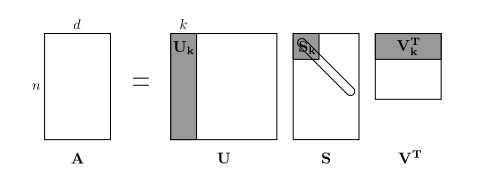
\includegraphics{imgs/svd.png}
\caption{Picture of an SVD}
\end{figure}

This reduced-dimensionality co-occurrence representation preserves
semantic relationships between words, e.g. \emph{doctor} and
\emph{hospital} will be closer than \emph{doctor} and \emph{dog}.

\textbf{Notes:} If you can barely remember what an eigenvalue is, here's
\href{https://davetang.org/file/Singular_Value_Decomposition_Tutorial.pdf}{a
slow, friendly introduction to SVD}. If you want to learn more
thoroughly about PCA or SVD, feel free to check out lectures
\href{https://web.stanford.edu/class/cs168/l/l7.pdf}{7},
\href{http://theory.stanford.edu/~tim/s15/l/l8.pdf}{8}, and
\href{https://web.stanford.edu/class/cs168/l/l9.pdf}{9} of CS168. These
course notes provide a great high-level treatment of these general
purpose algorithms. Though, for the purpose of this class, you only need
to know how to extract the k-dimensional embeddings by utilizing
pre-programmed implementations of these algorithms from the numpy,
scipy, or sklearn python packages. In practice, it is challenging to
apply full SVD to large corpora because of the memory needed to perform
PCA or SVD. However, if you only want the top \(k\) vector components
for relatively small \(k\) --- known as
\emph{\href{https://en.wikipedia.org/wiki/Singular_value_decomposition\#Truncated_SVD}{Truncated
SVD}} --- then there are reasonably scalable techniques to compute those
iteratively.

    \subsubsection{Plotting Co-Occurrence Word
Embeddings}\label{plotting-co-occurrence-word-embeddings}

Here, we will be using the Reuters (business and financial news) corpus.
If you haven't run the import cell at the top of this page, please run
it now (click it and press SHIFT-RETURN). The corpus consists of 10,788
news documents totaling 1.3 million words. These documents span 90
categories and are split into train and test. For more details, please
see https://www.nltk.org/book/ch02.html. We provide a
\texttt{read\_corpus} function below that pulls out only articles from
the "crude" (i.e. news articles about oil, gas, etc.) category. The
function also adds START and END tokens to each of the documents, and
lowercases words. You do \textbf{not} have perform any other kind of
pre-processing.

    \begin{Verbatim}[commandchars=\\\{\}]
{\color{incolor}In [{\color{incolor}3}]:} \PY{k}{def} \PY{n+nf}{read\PYZus{}corpus}\PY{p}{(}\PY{n}{category}\PY{o}{=}\PY{l+s+s2}{\PYZdq{}}\PY{l+s+s2}{crude}\PY{l+s+s2}{\PYZdq{}}\PY{p}{)}\PY{p}{:}
            \PY{l+s+sd}{\PYZdq{}\PYZdq{}\PYZdq{} Read files from the specified Reuter\PYZsq{}s category.}
        \PY{l+s+sd}{        Params:}
        \PY{l+s+sd}{            category (string): category name}
        \PY{l+s+sd}{        Return:}
        \PY{l+s+sd}{            list of lists, with words from each of the processed files}
        \PY{l+s+sd}{    \PYZdq{}\PYZdq{}\PYZdq{}}
            \PY{n}{files} \PY{o}{=} \PY{n}{reuters}\PY{o}{.}\PY{n}{fileids}\PY{p}{(}\PY{n}{category}\PY{p}{)}
            \PY{k}{return} \PY{p}{[}\PY{p}{[}\PY{n}{START\PYZus{}TOKEN}\PY{p}{]} \PY{o}{+} \PY{p}{[}\PY{n}{w}\PY{o}{.}\PY{n}{lower}\PY{p}{(}\PY{p}{)} \PY{k}{for} \PY{n}{w} \PY{o+ow}{in} \PY{n+nb}{list}\PY{p}{(}\PY{n}{reuters}\PY{o}{.}\PY{n}{words}\PY{p}{(}\PY{n}{f}\PY{p}{)}\PY{p}{)}\PY{p}{]} \PY{o}{+} \PY{p}{[}\PY{n}{END\PYZus{}TOKEN}\PY{p}{]} \PY{k}{for} \PY{n}{f} \PY{o+ow}{in} \PY{n}{files}\PY{p}{]}
\end{Verbatim}


    Let's have a look what these documents are like\ldots{}.

    \begin{Verbatim}[commandchars=\\\{\}]
{\color{incolor}In [{\color{incolor}4}]:} \PY{n}{reuters\PYZus{}corpus} \PY{o}{=} \PY{n}{read\PYZus{}corpus}\PY{p}{(}\PY{p}{)}
        \PY{n}{pprint}\PY{o}{.}\PY{n}{pprint}\PY{p}{(}\PY{n}{reuters\PYZus{}corpus}\PY{p}{[}\PY{p}{:}\PY{l+m+mi}{3}\PY{p}{]}\PY{p}{,} \PY{n}{compact}\PY{o}{=}\PY{k+kc}{True}\PY{p}{,} \PY{n}{width}\PY{o}{=}\PY{l+m+mi}{100}\PY{p}{)}
\end{Verbatim}


    \begin{Verbatim}[commandchars=\\\{\}]
[['<START>', 'japan', 'to', 'revise', 'long', '-', 'term', 'energy', 'demand', 'downwards', 'the',
  'ministry', 'of', 'international', 'trade', 'and', 'industry', '(', 'miti', ')', 'will', 'revise',
  'its', 'long', '-', 'term', 'energy', 'supply', '/', 'demand', 'outlook', 'by', 'august', 'to',
  'meet', 'a', 'forecast', 'downtrend', 'in', 'japanese', 'energy', 'demand', ',', 'ministry',
  'officials', 'said', '.', 'miti', 'is', 'expected', 'to', 'lower', 'the', 'projection', 'for',
  'primary', 'energy', 'supplies', 'in', 'the', 'year', '2000', 'to', '550', 'mln', 'kilolitres',
  '(', 'kl', ')', 'from', '600', 'mln', ',', 'they', 'said', '.', 'the', 'decision', 'follows',
  'the', 'emergence', 'of', 'structural', 'changes', 'in', 'japanese', 'industry', 'following',
  'the', 'rise', 'in', 'the', 'value', 'of', 'the', 'yen', 'and', 'a', 'decline', 'in', 'domestic',
  'electric', 'power', 'demand', '.', 'miti', 'is', 'planning', 'to', 'work', 'out', 'a', 'revised',
  'energy', 'supply', '/', 'demand', 'outlook', 'through', 'deliberations', 'of', 'committee',
  'meetings', 'of', 'the', 'agency', 'of', 'natural', 'resources', 'and', 'energy', ',', 'the',
  'officials', 'said', '.', 'they', 'said', 'miti', 'will', 'also', 'review', 'the', 'breakdown',
  'of', 'energy', 'supply', 'sources', ',', 'including', 'oil', ',', 'nuclear', ',', 'coal', 'and',
  'natural', 'gas', '.', 'nuclear', 'energy', 'provided', 'the', 'bulk', 'of', 'japan', "'", 's',
  'electric', 'power', 'in', 'the', 'fiscal', 'year', 'ended', 'march', '31', ',', 'supplying',
  'an', 'estimated', '27', 'pct', 'on', 'a', 'kilowatt', '/', 'hour', 'basis', ',', 'followed',
  'by', 'oil', '(', '23', 'pct', ')', 'and', 'liquefied', 'natural', 'gas', '(', '21', 'pct', '),',
  'they', 'noted', '.', '<END>'],
 ['<START>', 'energy', '/', 'u', '.', 's', '.', 'petrochemical', 'industry', 'cheap', 'oil',
  'feedstocks', ',', 'the', 'weakened', 'u', '.', 's', '.', 'dollar', 'and', 'a', 'plant',
  'utilization', 'rate', 'approaching', '90', 'pct', 'will', 'propel', 'the', 'streamlined', 'u',
  '.', 's', '.', 'petrochemical', 'industry', 'to', 'record', 'profits', 'this', 'year', ',',
  'with', 'growth', 'expected', 'through', 'at', 'least', '1990', ',', 'major', 'company',
  'executives', 'predicted', '.', 'this', 'bullish', 'outlook', 'for', 'chemical', 'manufacturing',
  'and', 'an', 'industrywide', 'move', 'to', 'shed', 'unrelated', 'businesses', 'has', 'prompted',
  'gaf', 'corp', '\&', 'lt', ';', 'gaf', '>,', 'privately', '-', 'held', 'cain', 'chemical', 'inc',
  ',', 'and', 'other', 'firms', 'to', 'aggressively', 'seek', 'acquisitions', 'of', 'petrochemical',
  'plants', '.', 'oil', 'companies', 'such', 'as', 'ashland', 'oil', 'inc', '\&', 'lt', ';', 'ash',
  '>,', 'the', 'kentucky', '-', 'based', 'oil', 'refiner', 'and', 'marketer', ',', 'are', 'also',
  'shopping', 'for', 'money', '-', 'making', 'petrochemical', 'businesses', 'to', 'buy', '.', '"',
  'i', 'see', 'us', 'poised', 'at', 'the', 'threshold', 'of', 'a', 'golden', 'period', ',"', 'said',
  'paul', 'oreffice', ',', 'chairman', 'of', 'giant', 'dow', 'chemical', 'co', '\&', 'lt', ';',
  'dow', '>,', 'adding', ',', '"', 'there', "'", 's', 'no', 'major', 'plant', 'capacity', 'being',
  'added', 'around', 'the', 'world', 'now', '.', 'the', 'whole', 'game', 'is', 'bringing', 'out',
  'new', 'products', 'and', 'improving', 'the', 'old', 'ones', '."', 'analysts', 'say', 'the',
  'chemical', 'industry', "'", 's', 'biggest', 'customers', ',', 'automobile', 'manufacturers',
  'and', 'home', 'builders', 'that', 'use', 'a', 'lot', 'of', 'paints', 'and', 'plastics', ',',
  'are', 'expected', 'to', 'buy', 'quantities', 'this', 'year', '.', 'u', '.', 's', '.',
  'petrochemical', 'plants', 'are', 'currently', 'operating', 'at', 'about', '90', 'pct',
  'capacity', ',', 'reflecting', 'tighter', 'supply', 'that', 'could', 'hike', 'product', 'prices',
  'by', '30', 'to', '40', 'pct', 'this', 'year', ',', 'said', 'john', 'dosher', ',', 'managing',
  'director', 'of', 'pace', 'consultants', 'inc', 'of', 'houston', '.', 'demand', 'for', 'some',
  'products', 'such', 'as', 'styrene', 'could', 'push', 'profit', 'margins', 'up', 'by', 'as',
  'much', 'as', '300', 'pct', ',', 'he', 'said', '.', 'oreffice', ',', 'speaking', 'at', 'a',
  'meeting', 'of', 'chemical', 'engineers', 'in', 'houston', ',', 'said', 'dow', 'would', 'easily',
  'top', 'the', '741', 'mln', 'dlrs', 'it', 'earned', 'last', 'year', 'and', 'predicted', 'it',
  'would', 'have', 'the', 'best', 'year', 'in', 'its', 'history', '.', 'in', '1985', ',', 'when',
  'oil', 'prices', 'were', 'still', 'above', '25', 'dlrs', 'a', 'barrel', 'and', 'chemical',
  'exports', 'were', 'adversely', 'affected', 'by', 'the', 'strong', 'u', '.', 's', '.', 'dollar',
  ',', 'dow', 'had', 'profits', 'of', '58', 'mln', 'dlrs', '.', '"', 'i', 'believe', 'the',
  'entire', 'chemical', 'industry', 'is', 'headed', 'for', 'a', 'record', 'year', 'or', 'close',
  'to', 'it', ',"', 'oreffice', 'said', '.', 'gaf', 'chairman', 'samuel', 'heyman', 'estimated',
  'that', 'the', 'u', '.', 's', '.', 'chemical', 'industry', 'would', 'report', 'a', '20', 'pct',
  'gain', 'in', 'profits', 'during', '1987', '.', 'last', 'year', ',', 'the', 'domestic',
  'industry', 'earned', 'a', 'total', 'of', '13', 'billion', 'dlrs', ',', 'a', '54', 'pct', 'leap',
  'from', '1985', '.', 'the', 'turn', 'in', 'the', 'fortunes', 'of', 'the', 'once', '-', 'sickly',
  'chemical', 'industry', 'has', 'been', 'brought', 'about', 'by', 'a', 'combination', 'of', 'luck',
  'and', 'planning', ',', 'said', 'pace', "'", 's', 'john', 'dosher', '.', 'dosher', 'said', 'last',
  'year', "'", 's', 'fall', 'in', 'oil', 'prices', 'made', 'feedstocks', 'dramatically', 'cheaper',
  'and', 'at', 'the', 'same', 'time', 'the', 'american', 'dollar', 'was', 'weakening', 'against',
  'foreign', 'currencies', '.', 'that', 'helped', 'boost', 'u', '.', 's', '.', 'chemical',
  'exports', '.', 'also', 'helping', 'to', 'bring', 'supply', 'and', 'demand', 'into', 'balance',
  'has', 'been', 'the', 'gradual', 'market', 'absorption', 'of', 'the', 'extra', 'chemical',
  'manufacturing', 'capacity', 'created', 'by', 'middle', 'eastern', 'oil', 'producers', 'in',
  'the', 'early', '1980s', '.', 'finally', ',', 'virtually', 'all', 'major', 'u', '.', 's', '.',
  'chemical', 'manufacturers', 'have', 'embarked', 'on', 'an', 'extensive', 'corporate',
  'restructuring', 'program', 'to', 'mothball', 'inefficient', 'plants', ',', 'trim', 'the',
  'payroll', 'and', 'eliminate', 'unrelated', 'businesses', '.', 'the', 'restructuring', 'touched',
  'off', 'a', 'flurry', 'of', 'friendly', 'and', 'hostile', 'takeover', 'attempts', '.', 'gaf', ',',
  'which', 'made', 'an', 'unsuccessful', 'attempt', 'in', '1985', 'to', 'acquire', 'union',
  'carbide', 'corp', '\&', 'lt', ';', 'uk', '>,', 'recently', 'offered', 'three', 'billion', 'dlrs',
  'for', 'borg', 'warner', 'corp', '\&', 'lt', ';', 'bor', '>,', 'a', 'chicago', 'manufacturer',
  'of', 'plastics', 'and', 'chemicals', '.', 'another', 'industry', 'powerhouse', ',', 'w', '.',
  'r', '.', 'grace', '\&', 'lt', ';', 'gra', '>', 'has', 'divested', 'its', 'retailing', ',',
  'restaurant', 'and', 'fertilizer', 'businesses', 'to', 'raise', 'cash', 'for', 'chemical',
  'acquisitions', '.', 'but', 'some', 'experts', 'worry', 'that', 'the', 'chemical', 'industry',
  'may', 'be', 'headed', 'for', 'trouble', 'if', 'companies', 'continue', 'turning', 'their',
  'back', 'on', 'the', 'manufacturing', 'of', 'staple', 'petrochemical', 'commodities', ',', 'such',
  'as', 'ethylene', ',', 'in', 'favor', 'of', 'more', 'profitable', 'specialty', 'chemicals',
  'that', 'are', 'custom', '-', 'designed', 'for', 'a', 'small', 'group', 'of', 'buyers', '.', '"',
  'companies', 'like', 'dupont', '\&', 'lt', ';', 'dd', '>', 'and', 'monsanto', 'co', '\&', 'lt', ';',
  'mtc', '>', 'spent', 'the', 'past', 'two', 'or', 'three', 'years', 'trying', 'to', 'get', 'out',
  'of', 'the', 'commodity', 'chemical', 'business', 'in', 'reaction', 'to', 'how', 'badly', 'the',
  'market', 'had', 'deteriorated', ',"', 'dosher', 'said', '.', '"', 'but', 'i', 'think', 'they',
  'will', 'eventually', 'kill', 'the', 'margins', 'on', 'the', 'profitable', 'chemicals', 'in',
  'the', 'niche', 'market', '."', 'some', 'top', 'chemical', 'executives', 'share', 'the',
  'concern', '.', '"', 'the', 'challenge', 'for', 'our', 'industry', 'is', 'to', 'keep', 'from',
  'getting', 'carried', 'away', 'and', 'repeating', 'past', 'mistakes', ',"', 'gaf', "'", 's',
  'heyman', 'cautioned', '.', '"', 'the', 'shift', 'from', 'commodity', 'chemicals', 'may', 'be',
  'ill', '-', 'advised', '.', 'specialty', 'businesses', 'do', 'not', 'stay', 'special', 'long',
  '."', 'houston', '-', 'based', 'cain', 'chemical', ',', 'created', 'this', 'month', 'by', 'the',
  'sterling', 'investment', 'banking', 'group', ',', 'believes', 'it', 'can', 'generate', '700',
  'mln', 'dlrs', 'in', 'annual', 'sales', 'by', 'bucking', 'the', 'industry', 'trend', '.',
  'chairman', 'gordon', 'cain', ',', 'who', 'previously', 'led', 'a', 'leveraged', 'buyout', 'of',
  'dupont', "'", 's', 'conoco', 'inc', "'", 's', 'chemical', 'business', ',', 'has', 'spent', '1',
  '.', '1', 'billion', 'dlrs', 'since', 'january', 'to', 'buy', 'seven', 'petrochemical', 'plants',
  'along', 'the', 'texas', 'gulf', 'coast', '.', 'the', 'plants', 'produce', 'only', 'basic',
  'commodity', 'petrochemicals', 'that', 'are', 'the', 'building', 'blocks', 'of', 'specialty',
  'products', '.', '"', 'this', 'kind', 'of', 'commodity', 'chemical', 'business', 'will', 'never',
  'be', 'a', 'glamorous', ',', 'high', '-', 'margin', 'business', ',"', 'cain', 'said', ',',
  'adding', 'that', 'demand', 'is', 'expected', 'to', 'grow', 'by', 'about', 'three', 'pct',
  'annually', '.', 'garo', 'armen', ',', 'an', 'analyst', 'with', 'dean', 'witter', 'reynolds', ',',
  'said', 'chemical', 'makers', 'have', 'also', 'benefitted', 'by', 'increasing', 'demand', 'for',
  'plastics', 'as', 'prices', 'become', 'more', 'competitive', 'with', 'aluminum', ',', 'wood',
  'and', 'steel', 'products', '.', 'armen', 'estimated', 'the', 'upturn', 'in', 'the', 'chemical',
  'business', 'could', 'last', 'as', 'long', 'as', 'four', 'or', 'five', 'years', ',', 'provided',
  'the', 'u', '.', 's', '.', 'economy', 'continues', 'its', 'modest', 'rate', 'of', 'growth', '.',
  '<END>'],
 ['<START>', 'turkey', 'calls', 'for', 'dialogue', 'to', 'solve', 'dispute', 'turkey', 'said',
  'today', 'its', 'disputes', 'with', 'greece', ',', 'including', 'rights', 'on', 'the',
  'continental', 'shelf', 'in', 'the', 'aegean', 'sea', ',', 'should', 'be', 'solved', 'through',
  'negotiations', '.', 'a', 'foreign', 'ministry', 'statement', 'said', 'the', 'latest', 'crisis',
  'between', 'the', 'two', 'nato', 'members', 'stemmed', 'from', 'the', 'continental', 'shelf',
  'dispute', 'and', 'an', 'agreement', 'on', 'this', 'issue', 'would', 'effect', 'the', 'security',
  ',', 'economy', 'and', 'other', 'rights', 'of', 'both', 'countries', '.', '"', 'as', 'the',
  'issue', 'is', 'basicly', 'political', ',', 'a', 'solution', 'can', 'only', 'be', 'found', 'by',
  'bilateral', 'negotiations', ',"', 'the', 'statement', 'said', '.', 'greece', 'has', 'repeatedly',
  'said', 'the', 'issue', 'was', 'legal', 'and', 'could', 'be', 'solved', 'at', 'the',
  'international', 'court', 'of', 'justice', '.', 'the', 'two', 'countries', 'approached', 'armed',
  'confrontation', 'last', 'month', 'after', 'greece', 'announced', 'it', 'planned', 'oil',
  'exploration', 'work', 'in', 'the', 'aegean', 'and', 'turkey', 'said', 'it', 'would', 'also',
  'search', 'for', 'oil', '.', 'a', 'face', '-', 'off', 'was', 'averted', 'when', 'turkey',
  'confined', 'its', 'research', 'to', 'territorrial', 'waters', '.', '"', 'the', 'latest',
  'crises', 'created', 'an', 'historic', 'opportunity', 'to', 'solve', 'the', 'disputes', 'between',
  'the', 'two', 'countries', ',"', 'the', 'foreign', 'ministry', 'statement', 'said', '.', 'turkey',
  "'", 's', 'ambassador', 'in', 'athens', ',', 'nazmi', 'akiman', ',', 'was', 'due', 'to', 'meet',
  'prime', 'minister', 'andreas', 'papandreou', 'today', 'for', 'the', 'greek', 'reply', 'to', 'a',
  'message', 'sent', 'last', 'week', 'by', 'turkish', 'prime', 'minister', 'turgut', 'ozal', '.',
  'the', 'contents', 'of', 'the', 'message', 'were', 'not', 'disclosed', '.', '<END>']]

    \end{Verbatim}

    \subsubsection{\texorpdfstring{Question 1.1: Implement
\texttt{distinct\_words} {[}code{]} (2
points)}{Question 1.1: Implement distinct\_words {[}code{]} (2 points)}}\label{question-1.1-implement-distinct_words-code-2-points}

Write a method to work out the distinct words (word types) that occur in
the corpus. You can do this with \texttt{for} loops, but it's more
efficient to do it with Python list comprehensions. In particular,
\href{https://coderwall.com/p/rcmaea/flatten-a-list-of-lists-in-one-line-in-python}{this}
may be useful to flatten a list of lists. If you're not familiar with
Python list comprehensions in general, here's
\href{https://python-3-patterns-idioms-test.readthedocs.io/en/latest/Comprehensions.html}{more
information}.

You may find it useful to use
\href{https://www.w3schools.com/python/python_sets.asp}{Python sets} to
remove duplicate words.

    \begin{Verbatim}[commandchars=\\\{\}]
{\color{incolor}In [{\color{incolor}5}]:} \PY{k}{def} \PY{n+nf}{distinct\PYZus{}words}\PY{p}{(}\PY{n}{corpus}\PY{p}{)}\PY{p}{:}
            \PY{l+s+sd}{\PYZdq{}\PYZdq{}\PYZdq{} Determine a list of distinct words for the corpus.}
        \PY{l+s+sd}{        Params:}
        \PY{l+s+sd}{            corpus (list of list of strings): corpus of documents}
        \PY{l+s+sd}{        Return:}
        \PY{l+s+sd}{            corpus\PYZus{}words (list of strings): list of distinct words across the corpus, sorted (using python \PYZsq{}sorted\PYZsq{} function)}
        \PY{l+s+sd}{            num\PYZus{}corpus\PYZus{}words (integer): number of distinct words across the corpus}
        \PY{l+s+sd}{    \PYZdq{}\PYZdq{}\PYZdq{}}
            \PY{n}{corpus\PYZus{}words} \PY{o}{=} \PY{p}{[}\PY{p}{]}
            \PY{n}{num\PYZus{}corpus\PYZus{}words} \PY{o}{=} \PY{o}{\PYZhy{}}\PY{l+m+mi}{1}
            
            \PY{c+c1}{\PYZsh{} \PYZhy{}\PYZhy{}\PYZhy{}\PYZhy{}\PYZhy{}\PYZhy{}\PYZhy{}\PYZhy{}\PYZhy{}\PYZhy{}\PYZhy{}\PYZhy{}\PYZhy{}\PYZhy{}\PYZhy{}\PYZhy{}\PYZhy{}\PYZhy{}}
            \PY{c+c1}{\PYZsh{} Write your implementation here.}
        
            \PY{n}{flattened\PYZus{}list} \PY{o}{=} \PY{p}{[}\PY{n}{word} \PY{k}{for} \PY{n}{i} \PY{o+ow}{in} \PY{n+nb}{range}\PY{p}{(}\PY{n+nb}{len}\PY{p}{(}\PY{n}{corpus}\PY{p}{)}\PY{p}{)} \PY{k}{for} \PY{n}{word} \PY{o+ow}{in} \PY{n}{corpus}\PY{p}{[}\PY{n}{i}\PY{p}{]}\PY{p}{]}
            
            \PY{n}{corpus\PYZus{}words} \PY{o}{=} \PY{n+nb}{sorted}\PY{p}{(}\PY{n+nb}{set}\PY{p}{(}\PY{n}{flattened\PYZus{}list}\PY{p}{)}\PY{p}{)}
            \PY{n}{num\PYZus{}corpus\PYZus{}words} \PY{o}{=} \PY{n+nb}{len}\PY{p}{(}\PY{n}{corpus\PYZus{}words}\PY{p}{)}
            
            \PY{c+c1}{\PYZsh{} \PYZhy{}\PYZhy{}\PYZhy{}\PYZhy{}\PYZhy{}\PYZhy{}\PYZhy{}\PYZhy{}\PYZhy{}\PYZhy{}\PYZhy{}\PYZhy{}\PYZhy{}\PYZhy{}\PYZhy{}\PYZhy{}\PYZhy{}\PYZhy{}}
        
            \PY{k}{return} \PY{n}{corpus\PYZus{}words}\PY{p}{,} \PY{n}{num\PYZus{}corpus\PYZus{}words}
\end{Verbatim}


    \begin{Verbatim}[commandchars=\\\{\}]
{\color{incolor}In [{\color{incolor}6}]:} \PY{c+c1}{\PYZsh{} \PYZhy{}\PYZhy{}\PYZhy{}\PYZhy{}\PYZhy{}\PYZhy{}\PYZhy{}\PYZhy{}\PYZhy{}\PYZhy{}\PYZhy{}\PYZhy{}\PYZhy{}\PYZhy{}\PYZhy{}\PYZhy{}\PYZhy{}\PYZhy{}\PYZhy{}\PYZhy{}\PYZhy{}}
        \PY{c+c1}{\PYZsh{} Run this sanity check}
        \PY{c+c1}{\PYZsh{} Note that this not an exhaustive check for correctness.}
        \PY{c+c1}{\PYZsh{} \PYZhy{}\PYZhy{}\PYZhy{}\PYZhy{}\PYZhy{}\PYZhy{}\PYZhy{}\PYZhy{}\PYZhy{}\PYZhy{}\PYZhy{}\PYZhy{}\PYZhy{}\PYZhy{}\PYZhy{}\PYZhy{}\PYZhy{}\PYZhy{}\PYZhy{}\PYZhy{}\PYZhy{}}
        
        \PY{c+c1}{\PYZsh{} Define toy corpus}
        \PY{n}{test\PYZus{}corpus} \PY{o}{=} \PY{p}{[}\PY{l+s+s2}{\PYZdq{}}\PY{l+s+s2}{START All that glitters isn}\PY{l+s+s2}{\PYZsq{}}\PY{l+s+s2}{t gold END}\PY{l+s+s2}{\PYZdq{}}\PY{o}{.}\PY{n}{split}\PY{p}{(}\PY{l+s+s2}{\PYZdq{}}\PY{l+s+s2}{ }\PY{l+s+s2}{\PYZdq{}}\PY{p}{)}\PY{p}{,} \PY{l+s+s2}{\PYZdq{}}\PY{l+s+s2}{START All}\PY{l+s+s2}{\PYZsq{}}\PY{l+s+s2}{s well that ends well END}\PY{l+s+s2}{\PYZdq{}}\PY{o}{.}\PY{n}{split}\PY{p}{(}\PY{l+s+s2}{\PYZdq{}}\PY{l+s+s2}{ }\PY{l+s+s2}{\PYZdq{}}\PY{p}{)}\PY{p}{]}
        \PY{n}{test\PYZus{}corpus\PYZus{}words}\PY{p}{,} \PY{n}{num\PYZus{}corpus\PYZus{}words} \PY{o}{=} \PY{n}{distinct\PYZus{}words}\PY{p}{(}\PY{n}{test\PYZus{}corpus}\PY{p}{)}
        
        \PY{c+c1}{\PYZsh{} Correct answers}
        \PY{n}{ans\PYZus{}test\PYZus{}corpus\PYZus{}words} \PY{o}{=} \PY{n+nb}{sorted}\PY{p}{(}\PY{n+nb}{list}\PY{p}{(}\PY{n+nb}{set}\PY{p}{(}\PY{p}{[}\PY{l+s+s2}{\PYZdq{}}\PY{l+s+s2}{START}\PY{l+s+s2}{\PYZdq{}}\PY{p}{,} \PY{l+s+s2}{\PYZdq{}}\PY{l+s+s2}{All}\PY{l+s+s2}{\PYZdq{}}\PY{p}{,} \PY{l+s+s2}{\PYZdq{}}\PY{l+s+s2}{ends}\PY{l+s+s2}{\PYZdq{}}\PY{p}{,} \PY{l+s+s2}{\PYZdq{}}\PY{l+s+s2}{that}\PY{l+s+s2}{\PYZdq{}}\PY{p}{,} \PY{l+s+s2}{\PYZdq{}}\PY{l+s+s2}{gold}\PY{l+s+s2}{\PYZdq{}}\PY{p}{,} \PY{l+s+s2}{\PYZdq{}}\PY{l+s+s2}{All}\PY{l+s+s2}{\PYZsq{}}\PY{l+s+s2}{s}\PY{l+s+s2}{\PYZdq{}}\PY{p}{,} \PY{l+s+s2}{\PYZdq{}}\PY{l+s+s2}{glitters}\PY{l+s+s2}{\PYZdq{}}\PY{p}{,} \PY{l+s+s2}{\PYZdq{}}\PY{l+s+s2}{isn}\PY{l+s+s2}{\PYZsq{}}\PY{l+s+s2}{t}\PY{l+s+s2}{\PYZdq{}}\PY{p}{,} \PY{l+s+s2}{\PYZdq{}}\PY{l+s+s2}{well}\PY{l+s+s2}{\PYZdq{}}\PY{p}{,} \PY{l+s+s2}{\PYZdq{}}\PY{l+s+s2}{END}\PY{l+s+s2}{\PYZdq{}}\PY{p}{]}\PY{p}{)}\PY{p}{)}\PY{p}{)}
        \PY{n}{ans\PYZus{}num\PYZus{}corpus\PYZus{}words} \PY{o}{=} \PY{n+nb}{len}\PY{p}{(}\PY{n}{ans\PYZus{}test\PYZus{}corpus\PYZus{}words}\PY{p}{)}
        
        \PY{c+c1}{\PYZsh{} Test correct number of words}
        \PY{k}{assert}\PY{p}{(}\PY{n}{num\PYZus{}corpus\PYZus{}words} \PY{o}{==} \PY{n}{ans\PYZus{}num\PYZus{}corpus\PYZus{}words}\PY{p}{)}\PY{p}{,} \PY{l+s+s2}{\PYZdq{}}\PY{l+s+s2}{Incorrect number of distinct words. Correct: }\PY{l+s+si}{\PYZob{}\PYZcb{}}\PY{l+s+s2}{. Yours: }\PY{l+s+si}{\PYZob{}\PYZcb{}}\PY{l+s+s2}{\PYZdq{}}\PY{o}{.}\PY{n}{format}\PY{p}{(}\PY{n}{ans\PYZus{}num\PYZus{}corpus\PYZus{}words}\PY{p}{,} \PY{n}{num\PYZus{}corpus\PYZus{}words}\PY{p}{)}
        
        \PY{c+c1}{\PYZsh{} Test correct words}
        \PY{k}{assert} \PY{p}{(}\PY{n}{test\PYZus{}corpus\PYZus{}words} \PY{o}{==} \PY{n}{ans\PYZus{}test\PYZus{}corpus\PYZus{}words}\PY{p}{)}\PY{p}{,} \PY{l+s+s2}{\PYZdq{}}\PY{l+s+s2}{Incorrect corpus\PYZus{}words.}\PY{l+s+se}{\PYZbs{}n}\PY{l+s+s2}{Correct: }\PY{l+s+si}{\PYZob{}\PYZcb{}}\PY{l+s+se}{\PYZbs{}n}\PY{l+s+s2}{Yours:   }\PY{l+s+si}{\PYZob{}\PYZcb{}}\PY{l+s+s2}{\PYZdq{}}\PY{o}{.}\PY{n}{format}\PY{p}{(}\PY{n+nb}{str}\PY{p}{(}\PY{n}{ans\PYZus{}test\PYZus{}corpus\PYZus{}words}\PY{p}{)}\PY{p}{,} \PY{n+nb}{str}\PY{p}{(}\PY{n}{test\PYZus{}corpus\PYZus{}words}\PY{p}{)}\PY{p}{)}
        
        \PY{c+c1}{\PYZsh{} Print Success}
        \PY{n+nb}{print} \PY{p}{(}\PY{l+s+s2}{\PYZdq{}}\PY{l+s+s2}{\PYZhy{}}\PY{l+s+s2}{\PYZdq{}} \PY{o}{*} \PY{l+m+mi}{80}\PY{p}{)}
        \PY{n+nb}{print}\PY{p}{(}\PY{l+s+s2}{\PYZdq{}}\PY{l+s+s2}{Passed All Tests!}\PY{l+s+s2}{\PYZdq{}}\PY{p}{)}
        \PY{n+nb}{print} \PY{p}{(}\PY{l+s+s2}{\PYZdq{}}\PY{l+s+s2}{\PYZhy{}}\PY{l+s+s2}{\PYZdq{}} \PY{o}{*} \PY{l+m+mi}{80}\PY{p}{)}
\end{Verbatim}


    \begin{Verbatim}[commandchars=\\\{\}]
--------------------------------------------------------------------------------
Passed All Tests!
--------------------------------------------------------------------------------

    \end{Verbatim}

    \subsubsection{\texorpdfstring{Question 1.2: Implement
\texttt{compute\_co\_occurrence\_matrix} {[}code{]} (3
points)}{Question 1.2: Implement compute\_co\_occurrence\_matrix {[}code{]} (3 points)}}\label{question-1.2-implement-compute_co_occurrence_matrix-code-3-points}

Write a method that constructs a co-occurrence matrix for a certain
window-size \(n\) (with a default of 4), considering words \(n\) before
and \(n\) after the word in the center of the window. Here, we start to
use \texttt{numpy\ (np)} to represent vectors, matrices, and tensors. If
you're not familiar with NumPy, there's a NumPy tutorial in the second
half of this cs231n
\href{http://cs231n.github.io/python-numpy-tutorial/}{Python NumPy
tutorial}.

    \begin{Verbatim}[commandchars=\\\{\}]
{\color{incolor}In [{\color{incolor}7}]:} \PY{k}{def} \PY{n+nf}{compute\PYZus{}co\PYZus{}occurrence\PYZus{}matrix}\PY{p}{(}\PY{n}{corpus}\PY{p}{,} \PY{n}{window\PYZus{}size}\PY{o}{=}\PY{l+m+mi}{4}\PY{p}{)}\PY{p}{:}
            \PY{l+s+sd}{\PYZdq{}\PYZdq{}\PYZdq{} Compute co\PYZhy{}occurrence matrix for the given corpus and window\PYZus{}size (default of 4).}
        \PY{l+s+sd}{    }
        \PY{l+s+sd}{        Note: Each word in a document should be at the center of a window. Words near edges will have a smaller}
        \PY{l+s+sd}{              number of co\PYZhy{}occurring words.}
        \PY{l+s+sd}{              }
        \PY{l+s+sd}{              For example, if we take the document \PYZdq{}START All that glitters is not gold END\PYZdq{} with window size of 4,}
        \PY{l+s+sd}{              \PYZdq{}All\PYZdq{} will co\PYZhy{}occur with \PYZdq{}START\PYZdq{}, \PYZdq{}that\PYZdq{}, \PYZdq{}glitters\PYZdq{}, \PYZdq{}is\PYZdq{}, and \PYZdq{}not\PYZdq{}.}
        \PY{l+s+sd}{    }
        \PY{l+s+sd}{        Params:}
        \PY{l+s+sd}{            corpus (list of list of strings): corpus of documents}
        \PY{l+s+sd}{            window\PYZus{}size (int): size of context window}
        \PY{l+s+sd}{        Return:}
        \PY{l+s+sd}{            M (numpy matrix of shape (number of unique words in the corpus , number of number of corpus words)): }
        \PY{l+s+sd}{                Co\PYZhy{}occurence matrix of word counts. }
        \PY{l+s+sd}{                The ordering of the words in the rows/columns should be the same as the ordering of the words given by the distinct\PYZus{}words function.}
        \PY{l+s+sd}{            word2Ind (dict): dictionary that maps word to index (i.e. row/column number) for matrix M.}
        \PY{l+s+sd}{    \PYZdq{}\PYZdq{}\PYZdq{}}
            \PY{n}{words}\PY{p}{,} \PY{n}{num\PYZus{}words} \PY{o}{=} \PY{n}{distinct\PYZus{}words}\PY{p}{(}\PY{n}{corpus}\PY{p}{)}
            \PY{n}{M} \PY{o}{=} \PY{k+kc}{None}
            \PY{n}{word2Ind} \PY{o}{=} \PY{p}{\PYZob{}}\PY{p}{\PYZcb{}}
            
            \PY{c+c1}{\PYZsh{} \PYZhy{}\PYZhy{}\PYZhy{}\PYZhy{}\PYZhy{}\PYZhy{}\PYZhy{}\PYZhy{}\PYZhy{}\PYZhy{}\PYZhy{}\PYZhy{}\PYZhy{}\PYZhy{}\PYZhy{}\PYZhy{}\PYZhy{}\PYZhy{}}
            \PY{c+c1}{\PYZsh{} Write your implementation here.}
        
            \PY{k}{for} \PY{n}{idx}\PY{p}{,} \PY{n}{word} \PY{o+ow}{in} \PY{n+nb}{enumerate}\PY{p}{(}\PY{n}{words}\PY{p}{)}\PY{p}{:}
                \PY{n}{word2Ind}\PY{p}{[}\PY{n}{word}\PY{p}{]} \PY{o}{=} \PY{n}{idx}
        
            \PY{n}{M} \PY{o}{=} \PY{n}{np}\PY{o}{.}\PY{n}{zeros}\PY{p}{(}\PY{p}{(}\PY{n}{num\PYZus{}words}\PY{p}{,} \PY{n}{num\PYZus{}words}\PY{p}{)}\PY{p}{)}
            
            \PY{k}{for} \PY{n}{line} \PY{o+ow}{in} \PY{n}{corpus}\PY{p}{:}
                \PY{k}{for} \PY{n}{i} \PY{o+ow}{in} \PY{n+nb}{range}\PY{p}{(}\PY{n+nb}{len}\PY{p}{(}\PY{n}{line}\PY{p}{)}\PY{p}{)}\PY{p}{:}
                    \PY{n}{i\PYZus{}idx} \PY{o}{=} \PY{n}{word2Ind}\PY{p}{[}\PY{n}{line}\PY{p}{[}\PY{n}{i}\PY{p}{]}\PY{p}{]}
                    
                    \PY{k}{for} \PY{n}{j} \PY{o+ow}{in} \PY{n+nb}{range}\PY{p}{(}\PY{n}{i}\PY{o}{\PYZhy{}}\PY{n}{window\PYZus{}size}\PY{p}{,} \PY{n}{i}\PY{o}{+}\PY{n}{window\PYZus{}size}\PY{o}{+}\PY{l+m+mi}{1}\PY{p}{)}\PY{p}{:}
                        
                        \PY{k}{if} \PY{n}{j} \PY{o}{\PYZlt{}} \PY{l+m+mi}{0} \PY{o+ow}{or} \PY{n}{j} \PY{o}{==} \PY{n}{i} \PY{o+ow}{or} \PY{n}{j} \PY{o}{\PYZgt{}}\PY{o}{=} \PY{n+nb}{len}\PY{p}{(}\PY{n}{line}\PY{p}{)}\PY{p}{:}
                            \PY{k}{continue}
                        
                        \PY{n}{j\PYZus{}idx} \PY{o}{=} \PY{n}{word2Ind}\PY{p}{[}\PY{n}{line}\PY{p}{[}\PY{n}{j}\PY{p}{]}\PY{p}{]}
                        \PY{n}{M}\PY{p}{[}\PY{n}{i\PYZus{}idx}\PY{p}{,} \PY{n}{j\PYZus{}idx}\PY{p}{]} \PY{o}{+}\PY{o}{=} \PY{l+m+mi}{1}
                        
                
            \PY{c+c1}{\PYZsh{} \PYZhy{}\PYZhy{}\PYZhy{}\PYZhy{}\PYZhy{}\PYZhy{}\PYZhy{}\PYZhy{}\PYZhy{}\PYZhy{}\PYZhy{}\PYZhy{}\PYZhy{}\PYZhy{}\PYZhy{}\PYZhy{}\PYZhy{}\PYZhy{}}
        
            \PY{k}{return} \PY{n}{M}\PY{p}{,} \PY{n}{word2Ind}
\end{Verbatim}


    \begin{Verbatim}[commandchars=\\\{\}]
{\color{incolor}In [{\color{incolor}8}]:} \PY{c+c1}{\PYZsh{} \PYZhy{}\PYZhy{}\PYZhy{}\PYZhy{}\PYZhy{}\PYZhy{}\PYZhy{}\PYZhy{}\PYZhy{}\PYZhy{}\PYZhy{}\PYZhy{}\PYZhy{}\PYZhy{}\PYZhy{}\PYZhy{}\PYZhy{}\PYZhy{}\PYZhy{}\PYZhy{}\PYZhy{}}
        \PY{c+c1}{\PYZsh{} Run this sanity check}
        \PY{c+c1}{\PYZsh{} Note that this is not an exhaustive check for correctness.}
        \PY{c+c1}{\PYZsh{} \PYZhy{}\PYZhy{}\PYZhy{}\PYZhy{}\PYZhy{}\PYZhy{}\PYZhy{}\PYZhy{}\PYZhy{}\PYZhy{}\PYZhy{}\PYZhy{}\PYZhy{}\PYZhy{}\PYZhy{}\PYZhy{}\PYZhy{}\PYZhy{}\PYZhy{}\PYZhy{}\PYZhy{}}
        
        \PY{c+c1}{\PYZsh{} Define toy corpus and get student\PYZsq{}s co\PYZhy{}occurrence matrix}
        \PY{n}{test\PYZus{}corpus} \PY{o}{=} \PY{p}{[}\PY{l+s+s2}{\PYZdq{}}\PY{l+s+s2}{START All that glitters isn}\PY{l+s+s2}{\PYZsq{}}\PY{l+s+s2}{t gold END}\PY{l+s+s2}{\PYZdq{}}\PY{o}{.}\PY{n}{split}\PY{p}{(}\PY{l+s+s2}{\PYZdq{}}\PY{l+s+s2}{ }\PY{l+s+s2}{\PYZdq{}}\PY{p}{)}\PY{p}{,} \PY{l+s+s2}{\PYZdq{}}\PY{l+s+s2}{START All}\PY{l+s+s2}{\PYZsq{}}\PY{l+s+s2}{s well that ends well END}\PY{l+s+s2}{\PYZdq{}}\PY{o}{.}\PY{n}{split}\PY{p}{(}\PY{l+s+s2}{\PYZdq{}}\PY{l+s+s2}{ }\PY{l+s+s2}{\PYZdq{}}\PY{p}{)}\PY{p}{]}
        \PY{n}{M\PYZus{}test}\PY{p}{,} \PY{n}{word2Ind\PYZus{}test} \PY{o}{=} \PY{n}{compute\PYZus{}co\PYZus{}occurrence\PYZus{}matrix}\PY{p}{(}\PY{n}{test\PYZus{}corpus}\PY{p}{,} \PY{n}{window\PYZus{}size}\PY{o}{=}\PY{l+m+mi}{1}\PY{p}{)}
        
        \PY{c+c1}{\PYZsh{} Correct M and word2Ind}
        \PY{n}{M\PYZus{}test\PYZus{}ans} \PY{o}{=} \PY{n}{np}\PY{o}{.}\PY{n}{array}\PY{p}{(} 
            \PY{p}{[}\PY{p}{[}\PY{l+m+mf}{0.}\PY{p}{,} \PY{l+m+mf}{0.}\PY{p}{,} \PY{l+m+mf}{0.}\PY{p}{,} \PY{l+m+mf}{1.}\PY{p}{,} \PY{l+m+mf}{0.}\PY{p}{,} \PY{l+m+mf}{0.}\PY{p}{,} \PY{l+m+mf}{0.}\PY{p}{,} \PY{l+m+mf}{0.}\PY{p}{,} \PY{l+m+mf}{1.}\PY{p}{,} \PY{l+m+mf}{0.}\PY{p}{,}\PY{p}{]}\PY{p}{,}
             \PY{p}{[}\PY{l+m+mf}{0.}\PY{p}{,} \PY{l+m+mf}{0.}\PY{p}{,} \PY{l+m+mf}{0.}\PY{p}{,} \PY{l+m+mf}{1.}\PY{p}{,} \PY{l+m+mf}{0.}\PY{p}{,} \PY{l+m+mf}{0.}\PY{p}{,} \PY{l+m+mf}{0.}\PY{p}{,} \PY{l+m+mf}{0.}\PY{p}{,} \PY{l+m+mf}{0.}\PY{p}{,} \PY{l+m+mf}{1.}\PY{p}{,}\PY{p}{]}\PY{p}{,}
             \PY{p}{[}\PY{l+m+mf}{0.}\PY{p}{,} \PY{l+m+mf}{0.}\PY{p}{,} \PY{l+m+mf}{0.}\PY{p}{,} \PY{l+m+mf}{0.}\PY{p}{,} \PY{l+m+mf}{0.}\PY{p}{,} \PY{l+m+mf}{0.}\PY{p}{,} \PY{l+m+mf}{1.}\PY{p}{,} \PY{l+m+mf}{0.}\PY{p}{,} \PY{l+m+mf}{0.}\PY{p}{,} \PY{l+m+mf}{1.}\PY{p}{,}\PY{p}{]}\PY{p}{,}
             \PY{p}{[}\PY{l+m+mf}{1.}\PY{p}{,} \PY{l+m+mf}{1.}\PY{p}{,} \PY{l+m+mf}{0.}\PY{p}{,} \PY{l+m+mf}{0.}\PY{p}{,} \PY{l+m+mf}{0.}\PY{p}{,} \PY{l+m+mf}{0.}\PY{p}{,} \PY{l+m+mf}{0.}\PY{p}{,} \PY{l+m+mf}{0.}\PY{p}{,} \PY{l+m+mf}{0.}\PY{p}{,} \PY{l+m+mf}{0.}\PY{p}{,}\PY{p}{]}\PY{p}{,}
             \PY{p}{[}\PY{l+m+mf}{0.}\PY{p}{,} \PY{l+m+mf}{0.}\PY{p}{,} \PY{l+m+mf}{0.}\PY{p}{,} \PY{l+m+mf}{0.}\PY{p}{,} \PY{l+m+mf}{0.}\PY{p}{,} \PY{l+m+mf}{0.}\PY{p}{,} \PY{l+m+mf}{0.}\PY{p}{,} \PY{l+m+mf}{0.}\PY{p}{,} \PY{l+m+mf}{1.}\PY{p}{,} \PY{l+m+mf}{1.}\PY{p}{,}\PY{p}{]}\PY{p}{,}
             \PY{p}{[}\PY{l+m+mf}{0.}\PY{p}{,} \PY{l+m+mf}{0.}\PY{p}{,} \PY{l+m+mf}{0.}\PY{p}{,} \PY{l+m+mf}{0.}\PY{p}{,} \PY{l+m+mf}{0.}\PY{p}{,} \PY{l+m+mf}{0.}\PY{p}{,} \PY{l+m+mf}{0.}\PY{p}{,} \PY{l+m+mf}{1.}\PY{p}{,} \PY{l+m+mf}{1.}\PY{p}{,} \PY{l+m+mf}{0.}\PY{p}{,}\PY{p}{]}\PY{p}{,}
             \PY{p}{[}\PY{l+m+mf}{0.}\PY{p}{,} \PY{l+m+mf}{0.}\PY{p}{,} \PY{l+m+mf}{1.}\PY{p}{,} \PY{l+m+mf}{0.}\PY{p}{,} \PY{l+m+mf}{0.}\PY{p}{,} \PY{l+m+mf}{0.}\PY{p}{,} \PY{l+m+mf}{0.}\PY{p}{,} \PY{l+m+mf}{1.}\PY{p}{,} \PY{l+m+mf}{0.}\PY{p}{,} \PY{l+m+mf}{0.}\PY{p}{,}\PY{p}{]}\PY{p}{,}
             \PY{p}{[}\PY{l+m+mf}{0.}\PY{p}{,} \PY{l+m+mf}{0.}\PY{p}{,} \PY{l+m+mf}{0.}\PY{p}{,} \PY{l+m+mf}{0.}\PY{p}{,} \PY{l+m+mf}{0.}\PY{p}{,} \PY{l+m+mf}{1.}\PY{p}{,} \PY{l+m+mf}{1.}\PY{p}{,} \PY{l+m+mf}{0.}\PY{p}{,} \PY{l+m+mf}{0.}\PY{p}{,} \PY{l+m+mf}{0.}\PY{p}{,}\PY{p}{]}\PY{p}{,}
             \PY{p}{[}\PY{l+m+mf}{1.}\PY{p}{,} \PY{l+m+mf}{0.}\PY{p}{,} \PY{l+m+mf}{0.}\PY{p}{,} \PY{l+m+mf}{0.}\PY{p}{,} \PY{l+m+mf}{1.}\PY{p}{,} \PY{l+m+mf}{1.}\PY{p}{,} \PY{l+m+mf}{0.}\PY{p}{,} \PY{l+m+mf}{0.}\PY{p}{,} \PY{l+m+mf}{0.}\PY{p}{,} \PY{l+m+mf}{1.}\PY{p}{,}\PY{p}{]}\PY{p}{,}
             \PY{p}{[}\PY{l+m+mf}{0.}\PY{p}{,} \PY{l+m+mf}{1.}\PY{p}{,} \PY{l+m+mf}{1.}\PY{p}{,} \PY{l+m+mf}{0.}\PY{p}{,} \PY{l+m+mf}{1.}\PY{p}{,} \PY{l+m+mf}{0.}\PY{p}{,} \PY{l+m+mf}{0.}\PY{p}{,} \PY{l+m+mf}{0.}\PY{p}{,} \PY{l+m+mf}{1.}\PY{p}{,} \PY{l+m+mf}{0.}\PY{p}{,}\PY{p}{]}\PY{p}{]}
        \PY{p}{)}
        \PY{n}{word2Ind\PYZus{}ans} \PY{o}{=} \PY{p}{\PYZob{}}\PY{l+s+s1}{\PYZsq{}}\PY{l+s+s1}{All}\PY{l+s+s1}{\PYZsq{}}\PY{p}{:} \PY{l+m+mi}{0}\PY{p}{,} \PY{l+s+s2}{\PYZdq{}}\PY{l+s+s2}{All}\PY{l+s+s2}{\PYZsq{}}\PY{l+s+s2}{s}\PY{l+s+s2}{\PYZdq{}}\PY{p}{:} \PY{l+m+mi}{1}\PY{p}{,} \PY{l+s+s1}{\PYZsq{}}\PY{l+s+s1}{END}\PY{l+s+s1}{\PYZsq{}}\PY{p}{:} \PY{l+m+mi}{2}\PY{p}{,} \PY{l+s+s1}{\PYZsq{}}\PY{l+s+s1}{START}\PY{l+s+s1}{\PYZsq{}}\PY{p}{:} \PY{l+m+mi}{3}\PY{p}{,} \PY{l+s+s1}{\PYZsq{}}\PY{l+s+s1}{ends}\PY{l+s+s1}{\PYZsq{}}\PY{p}{:} \PY{l+m+mi}{4}\PY{p}{,} \PY{l+s+s1}{\PYZsq{}}\PY{l+s+s1}{glitters}\PY{l+s+s1}{\PYZsq{}}\PY{p}{:} \PY{l+m+mi}{5}\PY{p}{,} \PY{l+s+s1}{\PYZsq{}}\PY{l+s+s1}{gold}\PY{l+s+s1}{\PYZsq{}}\PY{p}{:} \PY{l+m+mi}{6}\PY{p}{,} \PY{l+s+s2}{\PYZdq{}}\PY{l+s+s2}{isn}\PY{l+s+s2}{\PYZsq{}}\PY{l+s+s2}{t}\PY{l+s+s2}{\PYZdq{}}\PY{p}{:} \PY{l+m+mi}{7}\PY{p}{,} \PY{l+s+s1}{\PYZsq{}}\PY{l+s+s1}{that}\PY{l+s+s1}{\PYZsq{}}\PY{p}{:} \PY{l+m+mi}{8}\PY{p}{,} \PY{l+s+s1}{\PYZsq{}}\PY{l+s+s1}{well}\PY{l+s+s1}{\PYZsq{}}\PY{p}{:} \PY{l+m+mi}{9}\PY{p}{\PYZcb{}}
        
        \PY{c+c1}{\PYZsh{} Test correct word2Ind}
        \PY{k}{assert} \PY{p}{(}\PY{n}{word2Ind\PYZus{}ans} \PY{o}{==} \PY{n}{word2Ind\PYZus{}test}\PY{p}{)}\PY{p}{,} \PY{l+s+s2}{\PYZdq{}}\PY{l+s+s2}{Your word2Ind is incorrect:}\PY{l+s+se}{\PYZbs{}n}\PY{l+s+s2}{Correct: }\PY{l+s+si}{\PYZob{}\PYZcb{}}\PY{l+s+se}{\PYZbs{}n}\PY{l+s+s2}{Yours: }\PY{l+s+si}{\PYZob{}\PYZcb{}}\PY{l+s+s2}{\PYZdq{}}\PY{o}{.}\PY{n}{format}\PY{p}{(}\PY{n}{word2Ind\PYZus{}ans}\PY{p}{,} \PY{n}{word2Ind\PYZus{}test}\PY{p}{)}
        
        \PY{c+c1}{\PYZsh{} Test correct M shape}
        \PY{k}{assert} \PY{p}{(}\PY{n}{M\PYZus{}test}\PY{o}{.}\PY{n}{shape} \PY{o}{==} \PY{n}{M\PYZus{}test\PYZus{}ans}\PY{o}{.}\PY{n}{shape}\PY{p}{)}\PY{p}{,} \PY{l+s+s2}{\PYZdq{}}\PY{l+s+s2}{M matrix has incorrect shape.}\PY{l+s+se}{\PYZbs{}n}\PY{l+s+s2}{Correct: }\PY{l+s+si}{\PYZob{}\PYZcb{}}\PY{l+s+se}{\PYZbs{}n}\PY{l+s+s2}{Yours: }\PY{l+s+si}{\PYZob{}\PYZcb{}}\PY{l+s+s2}{\PYZdq{}}\PY{o}{.}\PY{n}{format}\PY{p}{(}\PY{n}{M\PYZus{}test}\PY{o}{.}\PY{n}{shape}\PY{p}{,} \PY{n}{M\PYZus{}test\PYZus{}ans}\PY{o}{.}\PY{n}{shape}\PY{p}{)}
        
        \PY{c+c1}{\PYZsh{} Test correct M values}
        \PY{k}{for} \PY{n}{w1} \PY{o+ow}{in} \PY{n}{word2Ind\PYZus{}ans}\PY{o}{.}\PY{n}{keys}\PY{p}{(}\PY{p}{)}\PY{p}{:}
            \PY{n}{idx1} \PY{o}{=} \PY{n}{word2Ind\PYZus{}ans}\PY{p}{[}\PY{n}{w1}\PY{p}{]}
            \PY{k}{for} \PY{n}{w2} \PY{o+ow}{in} \PY{n}{word2Ind\PYZus{}ans}\PY{o}{.}\PY{n}{keys}\PY{p}{(}\PY{p}{)}\PY{p}{:}
                \PY{n}{idx2} \PY{o}{=} \PY{n}{word2Ind\PYZus{}ans}\PY{p}{[}\PY{n}{w2}\PY{p}{]}
                \PY{n}{student} \PY{o}{=} \PY{n}{M\PYZus{}test}\PY{p}{[}\PY{n}{idx1}\PY{p}{,} \PY{n}{idx2}\PY{p}{]}
                \PY{n}{correct} \PY{o}{=} \PY{n}{M\PYZus{}test\PYZus{}ans}\PY{p}{[}\PY{n}{idx1}\PY{p}{,} \PY{n}{idx2}\PY{p}{]}
                \PY{k}{if} \PY{n}{student} \PY{o}{!=} \PY{n}{correct}\PY{p}{:}
                    \PY{n+nb}{print}\PY{p}{(}\PY{l+s+s2}{\PYZdq{}}\PY{l+s+s2}{Correct M:}\PY{l+s+s2}{\PYZdq{}}\PY{p}{)}
                    \PY{n+nb}{print}\PY{p}{(}\PY{n}{M\PYZus{}test\PYZus{}ans}\PY{p}{)}
                    \PY{n+nb}{print}\PY{p}{(}\PY{l+s+s2}{\PYZdq{}}\PY{l+s+s2}{Your M: }\PY{l+s+s2}{\PYZdq{}}\PY{p}{)}
                    \PY{n+nb}{print}\PY{p}{(}\PY{n}{M\PYZus{}test}\PY{p}{)}
                    \PY{k}{raise} \PY{n+ne}{AssertionError}\PY{p}{(}\PY{l+s+s2}{\PYZdq{}}\PY{l+s+s2}{Incorrect count at index (}\PY{l+s+si}{\PYZob{}\PYZcb{}}\PY{l+s+s2}{, }\PY{l+s+si}{\PYZob{}\PYZcb{}}\PY{l+s+s2}{)=(}\PY{l+s+si}{\PYZob{}\PYZcb{}}\PY{l+s+s2}{, }\PY{l+s+si}{\PYZob{}\PYZcb{}}\PY{l+s+s2}{) in matrix M. Yours has }\PY{l+s+si}{\PYZob{}\PYZcb{}}\PY{l+s+s2}{ but should have }\PY{l+s+si}{\PYZob{}\PYZcb{}}\PY{l+s+s2}{.}\PY{l+s+s2}{\PYZdq{}}\PY{o}{.}\PY{n}{format}\PY{p}{(}\PY{n}{idx1}\PY{p}{,} \PY{n}{idx2}\PY{p}{,} \PY{n}{w1}\PY{p}{,} \PY{n}{w2}\PY{p}{,} \PY{n}{student}\PY{p}{,} \PY{n}{correct}\PY{p}{)}\PY{p}{)}
        
        \PY{c+c1}{\PYZsh{} Print Success}
        \PY{n+nb}{print} \PY{p}{(}\PY{l+s+s2}{\PYZdq{}}\PY{l+s+s2}{\PYZhy{}}\PY{l+s+s2}{\PYZdq{}} \PY{o}{*} \PY{l+m+mi}{80}\PY{p}{)}
        \PY{n+nb}{print}\PY{p}{(}\PY{l+s+s2}{\PYZdq{}}\PY{l+s+s2}{Passed All Tests!}\PY{l+s+s2}{\PYZdq{}}\PY{p}{)}
        \PY{n+nb}{print} \PY{p}{(}\PY{l+s+s2}{\PYZdq{}}\PY{l+s+s2}{\PYZhy{}}\PY{l+s+s2}{\PYZdq{}} \PY{o}{*} \PY{l+m+mi}{80}\PY{p}{)}
\end{Verbatim}


    \begin{Verbatim}[commandchars=\\\{\}]
--------------------------------------------------------------------------------
Passed All Tests!
--------------------------------------------------------------------------------

    \end{Verbatim}

    \subsubsection{\texorpdfstring{Question 1.3: Implement
\texttt{reduce\_to\_k\_dim} {[}code{]} (1
point)}{Question 1.3: Implement reduce\_to\_k\_dim {[}code{]} (1 point)}}\label{question-1.3-implement-reduce_to_k_dim-code-1-point}

Construct a method that performs dimensionality reduction on the matrix
to produce k-dimensional embeddings. Use SVD to take the top k
components and produce a new matrix of k-dimensional embeddings.

\textbf{Note:} All of numpy, scipy, and scikit-learn (\texttt{sklearn})
provide \emph{some} implementation of SVD, but only scipy and sklearn
provide an implementation of Truncated SVD, and only sklearn provides an
efficient randomized algorithm for calculating large-scale Truncated
SVD. So please use
\href{https://scikit-learn.org/stable/modules/generated/sklearn.decomposition.TruncatedSVD.html}{sklearn.decomposition.TruncatedSVD}.

    \begin{Verbatim}[commandchars=\\\{\}]
{\color{incolor}In [{\color{incolor}9}]:} \PY{k}{def} \PY{n+nf}{reduce\PYZus{}to\PYZus{}k\PYZus{}dim}\PY{p}{(}\PY{n}{M}\PY{p}{,} \PY{n}{k}\PY{o}{=}\PY{l+m+mi}{2}\PY{p}{)}\PY{p}{:}
            \PY{l+s+sd}{\PYZdq{}\PYZdq{}\PYZdq{} Reduce a co\PYZhy{}occurence count matrix of dimensionality (num\PYZus{}corpus\PYZus{}words, num\PYZus{}corpus\PYZus{}words)}
        \PY{l+s+sd}{        to a matrix of dimensionality (num\PYZus{}corpus\PYZus{}words, k) using the following SVD function from Scikit\PYZhy{}Learn:}
        \PY{l+s+sd}{            \PYZhy{} http://scikit\PYZhy{}learn.org/stable/modules/generated/sklearn.decomposition.TruncatedSVD.html}
        \PY{l+s+sd}{    }
        \PY{l+s+sd}{        Params:}
        \PY{l+s+sd}{            M (numpy matrix of shape (number of unique words in the corpus , number of number of corpus words)): co\PYZhy{}occurence matrix of word counts}
        \PY{l+s+sd}{            k (int): embedding size of each word after dimension reduction}
        \PY{l+s+sd}{        Return:}
        \PY{l+s+sd}{            M\PYZus{}reduced (numpy matrix of shape (number of corpus words, k)): matrix of k\PYZhy{}dimensioal word embeddings.}
        \PY{l+s+sd}{                    In terms of the SVD from math class, this actually returns U * S}
        \PY{l+s+sd}{    \PYZdq{}\PYZdq{}\PYZdq{}}    
            \PY{n}{n\PYZus{}iters} \PY{o}{=} \PY{l+m+mi}{10}     \PY{c+c1}{\PYZsh{} Use this parameter in your call to `TruncatedSVD`}
            \PY{n}{M\PYZus{}reduced} \PY{o}{=} \PY{k+kc}{None}
            \PY{n+nb}{print}\PY{p}{(}\PY{l+s+s2}{\PYZdq{}}\PY{l+s+s2}{Running Truncated SVD over }\PY{l+s+si}{\PYZpc{}i}\PY{l+s+s2}{ words...}\PY{l+s+s2}{\PYZdq{}} \PY{o}{\PYZpc{}} \PY{p}{(}\PY{n}{M}\PY{o}{.}\PY{n}{shape}\PY{p}{[}\PY{l+m+mi}{0}\PY{p}{]}\PY{p}{)}\PY{p}{)}
            
                \PY{c+c1}{\PYZsh{} \PYZhy{}\PYZhy{}\PYZhy{}\PYZhy{}\PYZhy{}\PYZhy{}\PYZhy{}\PYZhy{}\PYZhy{}\PYZhy{}\PYZhy{}\PYZhy{}\PYZhy{}\PYZhy{}\PYZhy{}\PYZhy{}\PYZhy{}\PYZhy{}}
                \PY{c+c1}{\PYZsh{} Write your implementation here.}
            
            \PY{n}{svd} \PY{o}{=} \PY{n}{TruncatedSVD}\PY{p}{(}\PY{n}{n\PYZus{}components}\PY{o}{=}\PY{n}{k}\PY{p}{,} \PY{n}{n\PYZus{}iter}\PY{o}{=}\PY{n}{n\PYZus{}iters}\PY{p}{)}
            \PY{n}{M\PYZus{}reduced} \PY{o}{=} \PY{n}{svd}\PY{o}{.}\PY{n}{fit\PYZus{}transform}\PY{p}{(}\PY{n}{M}\PY{p}{)}
        
                \PY{c+c1}{\PYZsh{} \PYZhy{}\PYZhy{}\PYZhy{}\PYZhy{}\PYZhy{}\PYZhy{}\PYZhy{}\PYZhy{}\PYZhy{}\PYZhy{}\PYZhy{}\PYZhy{}\PYZhy{}\PYZhy{}\PYZhy{}\PYZhy{}\PYZhy{}\PYZhy{}}
        
            \PY{n+nb}{print}\PY{p}{(}\PY{l+s+s2}{\PYZdq{}}\PY{l+s+s2}{Done.}\PY{l+s+s2}{\PYZdq{}}\PY{p}{)}
            \PY{k}{return} \PY{n}{M\PYZus{}reduced}
\end{Verbatim}


    \begin{Verbatim}[commandchars=\\\{\}]
{\color{incolor}In [{\color{incolor}10}]:} \PY{c+c1}{\PYZsh{} \PYZhy{}\PYZhy{}\PYZhy{}\PYZhy{}\PYZhy{}\PYZhy{}\PYZhy{}\PYZhy{}\PYZhy{}\PYZhy{}\PYZhy{}\PYZhy{}\PYZhy{}\PYZhy{}\PYZhy{}\PYZhy{}\PYZhy{}\PYZhy{}\PYZhy{}\PYZhy{}\PYZhy{}}
         \PY{c+c1}{\PYZsh{} Run this sanity check}
         \PY{c+c1}{\PYZsh{} Note that this not an exhaustive check for correctness }
         \PY{c+c1}{\PYZsh{} In fact we only check that your M\PYZus{}reduced has the right dimensions.}
         \PY{c+c1}{\PYZsh{} \PYZhy{}\PYZhy{}\PYZhy{}\PYZhy{}\PYZhy{}\PYZhy{}\PYZhy{}\PYZhy{}\PYZhy{}\PYZhy{}\PYZhy{}\PYZhy{}\PYZhy{}\PYZhy{}\PYZhy{}\PYZhy{}\PYZhy{}\PYZhy{}\PYZhy{}\PYZhy{}\PYZhy{}}
         
         \PY{c+c1}{\PYZsh{} Define toy corpus and run student code}
         \PY{n}{test\PYZus{}corpus} \PY{o}{=} \PY{p}{[}\PY{l+s+s2}{\PYZdq{}}\PY{l+s+s2}{START All that glitters isn}\PY{l+s+s2}{\PYZsq{}}\PY{l+s+s2}{t gold END}\PY{l+s+s2}{\PYZdq{}}\PY{o}{.}\PY{n}{split}\PY{p}{(}\PY{l+s+s2}{\PYZdq{}}\PY{l+s+s2}{ }\PY{l+s+s2}{\PYZdq{}}\PY{p}{)}\PY{p}{,} \PY{l+s+s2}{\PYZdq{}}\PY{l+s+s2}{START All}\PY{l+s+s2}{\PYZsq{}}\PY{l+s+s2}{s well that ends well END}\PY{l+s+s2}{\PYZdq{}}\PY{o}{.}\PY{n}{split}\PY{p}{(}\PY{l+s+s2}{\PYZdq{}}\PY{l+s+s2}{ }\PY{l+s+s2}{\PYZdq{}}\PY{p}{)}\PY{p}{]}
         \PY{n}{M\PYZus{}test}\PY{p}{,} \PY{n}{word2Ind\PYZus{}test} \PY{o}{=} \PY{n}{compute\PYZus{}co\PYZus{}occurrence\PYZus{}matrix}\PY{p}{(}\PY{n}{test\PYZus{}corpus}\PY{p}{,} \PY{n}{window\PYZus{}size}\PY{o}{=}\PY{l+m+mi}{1}\PY{p}{)}
         \PY{n}{M\PYZus{}test\PYZus{}reduced} \PY{o}{=} \PY{n}{reduce\PYZus{}to\PYZus{}k\PYZus{}dim}\PY{p}{(}\PY{n}{M\PYZus{}test}\PY{p}{,} \PY{n}{k}\PY{o}{=}\PY{l+m+mi}{2}\PY{p}{)}
         
         \PY{c+c1}{\PYZsh{} Test proper dimensions}
         \PY{k}{assert} \PY{p}{(}\PY{n}{M\PYZus{}test\PYZus{}reduced}\PY{o}{.}\PY{n}{shape}\PY{p}{[}\PY{l+m+mi}{0}\PY{p}{]} \PY{o}{==} \PY{l+m+mi}{10}\PY{p}{)}\PY{p}{,} \PY{l+s+s2}{\PYZdq{}}\PY{l+s+s2}{M\PYZus{}reduced has }\PY{l+s+si}{\PYZob{}\PYZcb{}}\PY{l+s+s2}{ rows; should have }\PY{l+s+si}{\PYZob{}\PYZcb{}}\PY{l+s+s2}{\PYZdq{}}\PY{o}{.}\PY{n}{format}\PY{p}{(}\PY{n}{M\PYZus{}test\PYZus{}reduced}\PY{o}{.}\PY{n}{shape}\PY{p}{[}\PY{l+m+mi}{0}\PY{p}{]}\PY{p}{,} \PY{l+m+mi}{10}\PY{p}{)}
         \PY{k}{assert} \PY{p}{(}\PY{n}{M\PYZus{}test\PYZus{}reduced}\PY{o}{.}\PY{n}{shape}\PY{p}{[}\PY{l+m+mi}{1}\PY{p}{]} \PY{o}{==} \PY{l+m+mi}{2}\PY{p}{)}\PY{p}{,} \PY{l+s+s2}{\PYZdq{}}\PY{l+s+s2}{M\PYZus{}reduced has }\PY{l+s+si}{\PYZob{}\PYZcb{}}\PY{l+s+s2}{ columns; should have }\PY{l+s+si}{\PYZob{}\PYZcb{}}\PY{l+s+s2}{\PYZdq{}}\PY{o}{.}\PY{n}{format}\PY{p}{(}\PY{n}{M\PYZus{}test\PYZus{}reduced}\PY{o}{.}\PY{n}{shape}\PY{p}{[}\PY{l+m+mi}{1}\PY{p}{]}\PY{p}{,} \PY{l+m+mi}{2}\PY{p}{)}
         
         \PY{c+c1}{\PYZsh{} Print Success}
         \PY{n+nb}{print} \PY{p}{(}\PY{l+s+s2}{\PYZdq{}}\PY{l+s+s2}{\PYZhy{}}\PY{l+s+s2}{\PYZdq{}} \PY{o}{*} \PY{l+m+mi}{80}\PY{p}{)}
         \PY{n+nb}{print}\PY{p}{(}\PY{l+s+s2}{\PYZdq{}}\PY{l+s+s2}{Passed All Tests!}\PY{l+s+s2}{\PYZdq{}}\PY{p}{)}
         \PY{n+nb}{print} \PY{p}{(}\PY{l+s+s2}{\PYZdq{}}\PY{l+s+s2}{\PYZhy{}}\PY{l+s+s2}{\PYZdq{}} \PY{o}{*} \PY{l+m+mi}{80}\PY{p}{)}
\end{Verbatim}


    \begin{Verbatim}[commandchars=\\\{\}]
Running Truncated SVD over 10 words{\ldots}
Done.
--------------------------------------------------------------------------------
Passed All Tests!
--------------------------------------------------------------------------------

    \end{Verbatim}

    \subsubsection{\texorpdfstring{Question 1.4: Implement
\texttt{plot\_embeddings} {[}code{]} (1
point)}{Question 1.4: Implement plot\_embeddings {[}code{]} (1 point)}}\label{question-1.4-implement-plot_embeddings-code-1-point}

Here you will write a function to plot a set of 2D vectors in 2D space.
For graphs, we will use Matplotlib (\texttt{plt}).

For this example, you may find it useful to adapt
\href{https://www.pythonmembers.club/2018/05/08/matplotlib-scatter-plot-annotate-set-text-at-label-each-point/}{this
code}. In the future, a good way to make a plot is to look at
\href{https://matplotlib.org/gallery/index.html}{the Matplotlib
gallery}, find a plot that looks somewhat like what you want, and adapt
the code they give.

    \begin{Verbatim}[commandchars=\\\{\}]
{\color{incolor}In [{\color{incolor}11}]:} \PY{k}{def} \PY{n+nf}{plot\PYZus{}embeddings}\PY{p}{(}\PY{n}{M\PYZus{}reduced}\PY{p}{,} \PY{n}{word2Ind}\PY{p}{,} \PY{n}{words}\PY{p}{)}\PY{p}{:}
             \PY{l+s+sd}{\PYZdq{}\PYZdq{}\PYZdq{} Plot in a scatterplot the embeddings of the words specified in the list \PYZdq{}words\PYZdq{}.}
         \PY{l+s+sd}{        NOTE: do not plot all the words listed in M\PYZus{}reduced / word2Ind.}
         \PY{l+s+sd}{        Include a label next to each point.}
         \PY{l+s+sd}{        }
         \PY{l+s+sd}{        Params:}
         \PY{l+s+sd}{            M\PYZus{}reduced (numpy matrix of shape (number of unique words in the corpus , k)): matrix of k\PYZhy{}dimensioal word embeddings}
         \PY{l+s+sd}{            word2Ind (dict): dictionary that maps word to indices for matrix M}
         \PY{l+s+sd}{            words (list of strings): words whose embeddings we want to visualize}
         \PY{l+s+sd}{    \PYZdq{}\PYZdq{}\PYZdq{}}
         
             \PY{c+c1}{\PYZsh{} \PYZhy{}\PYZhy{}\PYZhy{}\PYZhy{}\PYZhy{}\PYZhy{}\PYZhy{}\PYZhy{}\PYZhy{}\PYZhy{}\PYZhy{}\PYZhy{}\PYZhy{}\PYZhy{}\PYZhy{}\PYZhy{}\PYZhy{}\PYZhy{}}
             \PY{c+c1}{\PYZsh{} Write your implementation here.}
         
             \PY{k}{for} \PY{n}{i}\PY{p}{,} \PY{n}{word} \PY{o+ow}{in} \PY{n+nb}{enumerate}\PY{p}{(}\PY{n}{words}\PY{p}{)}\PY{p}{:}
                 
                 \PY{n}{word\PYZus{}idx} \PY{o}{=} \PY{n}{word2Ind}\PY{p}{[}\PY{n}{word}\PY{p}{]}
                 \PY{n}{word\PYZus{}vec} \PY{o}{=} \PY{n}{M\PYZus{}reduced}\PY{p}{[}\PY{n}{word\PYZus{}idx}\PY{p}{]}
                 
                 \PY{n}{x} \PY{o}{=} \PY{n}{word\PYZus{}vec}\PY{p}{[}\PY{l+m+mi}{0}\PY{p}{]}
                 \PY{n}{y} \PY{o}{=} \PY{n}{word\PYZus{}vec}\PY{p}{[}\PY{l+m+mi}{1}\PY{p}{]}
                 \PY{n}{plt}\PY{o}{.}\PY{n}{scatter}\PY{p}{(}\PY{n}{x}\PY{p}{,} \PY{n}{y}\PY{p}{,} \PY{n}{marker}\PY{o}{=}\PY{l+s+s1}{\PYZsq{}}\PY{l+s+s1}{x}\PY{l+s+s1}{\PYZsq{}}\PY{p}{,} \PY{n}{color}\PY{o}{=}\PY{l+s+s1}{\PYZsq{}}\PY{l+s+s1}{red}\PY{l+s+s1}{\PYZsq{}}\PY{p}{)}
                 \PY{n}{plt}\PY{o}{.}\PY{n}{text}\PY{p}{(}\PY{n}{x}\PY{o}{+}\PY{l+m+mf}{0.001}\PY{p}{,} \PY{n}{y}\PY{o}{+}\PY{l+m+mf}{0.001}\PY{p}{,} \PY{n}{word}\PY{p}{,} \PY{n}{fontsize}\PY{o}{=}\PY{l+m+mi}{9}\PY{p}{)}
                 
             \PY{n}{plt}\PY{o}{.}\PY{n}{show}\PY{p}{(}\PY{p}{)}
             
             \PY{c+c1}{\PYZsh{} \PYZhy{}\PYZhy{}\PYZhy{}\PYZhy{}\PYZhy{}\PYZhy{}\PYZhy{}\PYZhy{}\PYZhy{}\PYZhy{}\PYZhy{}\PYZhy{}\PYZhy{}\PYZhy{}\PYZhy{}\PYZhy{}\PYZhy{}\PYZhy{}}
\end{Verbatim}


    \begin{Verbatim}[commandchars=\\\{\}]
{\color{incolor}In [{\color{incolor}12}]:} \PY{c+c1}{\PYZsh{} \PYZhy{}\PYZhy{}\PYZhy{}\PYZhy{}\PYZhy{}\PYZhy{}\PYZhy{}\PYZhy{}\PYZhy{}\PYZhy{}\PYZhy{}\PYZhy{}\PYZhy{}\PYZhy{}\PYZhy{}\PYZhy{}\PYZhy{}\PYZhy{}\PYZhy{}\PYZhy{}\PYZhy{}}
         \PY{c+c1}{\PYZsh{} Run this sanity check}
         \PY{c+c1}{\PYZsh{} Note that this not an exhaustive check for correctness.}
         \PY{c+c1}{\PYZsh{} The plot produced should look like the \PYZdq{}test solution plot\PYZdq{} depicted below. }
         \PY{c+c1}{\PYZsh{} \PYZhy{}\PYZhy{}\PYZhy{}\PYZhy{}\PYZhy{}\PYZhy{}\PYZhy{}\PYZhy{}\PYZhy{}\PYZhy{}\PYZhy{}\PYZhy{}\PYZhy{}\PYZhy{}\PYZhy{}\PYZhy{}\PYZhy{}\PYZhy{}\PYZhy{}\PYZhy{}\PYZhy{}}
         
         \PY{n+nb}{print} \PY{p}{(}\PY{l+s+s2}{\PYZdq{}}\PY{l+s+s2}{\PYZhy{}}\PY{l+s+s2}{\PYZdq{}} \PY{o}{*} \PY{l+m+mi}{80}\PY{p}{)}
         \PY{n+nb}{print} \PY{p}{(}\PY{l+s+s2}{\PYZdq{}}\PY{l+s+s2}{Outputted Plot:}\PY{l+s+s2}{\PYZdq{}}\PY{p}{)}
         
         \PY{n}{M\PYZus{}reduced\PYZus{}plot\PYZus{}test} \PY{o}{=} \PY{n}{np}\PY{o}{.}\PY{n}{array}\PY{p}{(}\PY{p}{[}\PY{p}{[}\PY{l+m+mi}{1}\PY{p}{,} \PY{l+m+mi}{1}\PY{p}{]}\PY{p}{,} \PY{p}{[}\PY{o}{\PYZhy{}}\PY{l+m+mi}{1}\PY{p}{,} \PY{o}{\PYZhy{}}\PY{l+m+mi}{1}\PY{p}{]}\PY{p}{,} \PY{p}{[}\PY{l+m+mi}{1}\PY{p}{,} \PY{o}{\PYZhy{}}\PY{l+m+mi}{1}\PY{p}{]}\PY{p}{,} \PY{p}{[}\PY{o}{\PYZhy{}}\PY{l+m+mi}{1}\PY{p}{,} \PY{l+m+mi}{1}\PY{p}{]}\PY{p}{,} \PY{p}{[}\PY{l+m+mi}{0}\PY{p}{,} \PY{l+m+mi}{0}\PY{p}{]}\PY{p}{]}\PY{p}{)}
         \PY{n}{word2Ind\PYZus{}plot\PYZus{}test} \PY{o}{=} \PY{p}{\PYZob{}}\PY{l+s+s1}{\PYZsq{}}\PY{l+s+s1}{test1}\PY{l+s+s1}{\PYZsq{}}\PY{p}{:} \PY{l+m+mi}{0}\PY{p}{,} \PY{l+s+s1}{\PYZsq{}}\PY{l+s+s1}{test2}\PY{l+s+s1}{\PYZsq{}}\PY{p}{:} \PY{l+m+mi}{1}\PY{p}{,} \PY{l+s+s1}{\PYZsq{}}\PY{l+s+s1}{test3}\PY{l+s+s1}{\PYZsq{}}\PY{p}{:} \PY{l+m+mi}{2}\PY{p}{,} \PY{l+s+s1}{\PYZsq{}}\PY{l+s+s1}{test4}\PY{l+s+s1}{\PYZsq{}}\PY{p}{:} \PY{l+m+mi}{3}\PY{p}{,} \PY{l+s+s1}{\PYZsq{}}\PY{l+s+s1}{test5}\PY{l+s+s1}{\PYZsq{}}\PY{p}{:} \PY{l+m+mi}{4}\PY{p}{\PYZcb{}}
         \PY{n}{words} \PY{o}{=} \PY{p}{[}\PY{l+s+s1}{\PYZsq{}}\PY{l+s+s1}{test1}\PY{l+s+s1}{\PYZsq{}}\PY{p}{,} \PY{l+s+s1}{\PYZsq{}}\PY{l+s+s1}{test2}\PY{l+s+s1}{\PYZsq{}}\PY{p}{,} \PY{l+s+s1}{\PYZsq{}}\PY{l+s+s1}{test3}\PY{l+s+s1}{\PYZsq{}}\PY{p}{,} \PY{l+s+s1}{\PYZsq{}}\PY{l+s+s1}{test4}\PY{l+s+s1}{\PYZsq{}}\PY{p}{,} \PY{l+s+s1}{\PYZsq{}}\PY{l+s+s1}{test5}\PY{l+s+s1}{\PYZsq{}}\PY{p}{]}
         \PY{n}{plot\PYZus{}embeddings}\PY{p}{(}\PY{n}{M\PYZus{}reduced\PYZus{}plot\PYZus{}test}\PY{p}{,} \PY{n}{word2Ind\PYZus{}plot\PYZus{}test}\PY{p}{,} \PY{n}{words}\PY{p}{)}
         
         \PY{n+nb}{print} \PY{p}{(}\PY{l+s+s2}{\PYZdq{}}\PY{l+s+s2}{\PYZhy{}}\PY{l+s+s2}{\PYZdq{}} \PY{o}{*} \PY{l+m+mi}{80}\PY{p}{)}
\end{Verbatim}


    \begin{Verbatim}[commandchars=\\\{\}]
--------------------------------------------------------------------------------
Outputted Plot:

    \end{Verbatim}

    \begin{center}
    \adjustimage{max size={0.9\linewidth}{0.9\paperheight}}{output_20_1.png}
    \end{center}
    { \hspace*{\fill} \\}
    
    \begin{Verbatim}[commandchars=\\\{\}]
--------------------------------------------------------------------------------

    \end{Verbatim}

    \textbf{Test Plot Solution} 

    \subsubsection{Question 1.5: Co-Occurrence Plot Analysis {[}written{]}
(3
points)}\label{question-1.5-co-occurrence-plot-analysis-written-3-points}

Now we will put together all the parts you have written! We will compute
the co-occurrence matrix with fixed window of 5, over the Reuters
"crude" corpus. Then we will use TruncatedSVD to compute 2-dimensional
embeddings of each word. TruncatedSVD returns U*S, so we normalize the
returned vectors, so that all the vectors will appear around the unit
circle (therefore closeness is directional closeness). \textbf{Note}:
The line of code below that does the normalizing uses the NumPy concept
of \emph{broadcasting}. If you don't know about broadcasting, check out
\href{https://jakevdp.github.io/PythonDataScienceHandbook/02.05-computation-on-arrays-broadcasting.html}{Computation
on Arrays: Broadcasting by Jake VanderPlas}.

Run the below cell to produce the plot. It'll probably take a few
seconds to run. What clusters together in 2-dimensional embedding space?
What doesn't cluster together that you might think should have?
\textbf{Note:} "bpd" stands for "barrels per day" and is a commonly used
abbreviation in crude oil topic articles.

    \begin{Verbatim}[commandchars=\\\{\}]
{\color{incolor}In [{\color{incolor}13}]:} \PY{c+c1}{\PYZsh{} \PYZhy{}\PYZhy{}\PYZhy{}\PYZhy{}\PYZhy{}\PYZhy{}\PYZhy{}\PYZhy{}\PYZhy{}\PYZhy{}\PYZhy{}\PYZhy{}\PYZhy{}\PYZhy{}\PYZhy{}\PYZhy{}\PYZhy{}\PYZhy{}\PYZhy{}\PYZhy{}\PYZhy{}\PYZhy{}\PYZhy{}\PYZhy{}\PYZhy{}\PYZhy{}\PYZhy{}\PYZhy{}\PYZhy{}}
         \PY{c+c1}{\PYZsh{} Run This Cell to Produce Your Plot}
         \PY{c+c1}{\PYZsh{} \PYZhy{}\PYZhy{}\PYZhy{}\PYZhy{}\PYZhy{}\PYZhy{}\PYZhy{}\PYZhy{}\PYZhy{}\PYZhy{}\PYZhy{}\PYZhy{}\PYZhy{}\PYZhy{}\PYZhy{}\PYZhy{}\PYZhy{}\PYZhy{}\PYZhy{}\PYZhy{}\PYZhy{}\PYZhy{}\PYZhy{}\PYZhy{}\PYZhy{}\PYZhy{}\PYZhy{}\PYZhy{}\PYZhy{}\PYZhy{}}
         \PY{n}{reuters\PYZus{}corpus} \PY{o}{=} \PY{n}{read\PYZus{}corpus}\PY{p}{(}\PY{p}{)}
         \PY{n}{M\PYZus{}co\PYZus{}occurrence}\PY{p}{,} \PY{n}{word2Ind\PYZus{}co\PYZus{}occurrence} \PY{o}{=} \PY{n}{compute\PYZus{}co\PYZus{}occurrence\PYZus{}matrix}\PY{p}{(}\PY{n}{reuters\PYZus{}corpus}\PY{p}{)}
         \PY{n}{M\PYZus{}reduced\PYZus{}co\PYZus{}occurrence} \PY{o}{=} \PY{n}{reduce\PYZus{}to\PYZus{}k\PYZus{}dim}\PY{p}{(}\PY{n}{M\PYZus{}co\PYZus{}occurrence}\PY{p}{,} \PY{n}{k}\PY{o}{=}\PY{l+m+mi}{2}\PY{p}{)}
         
         \PY{c+c1}{\PYZsh{} Rescale (normalize) the rows to make them each of unit\PYZhy{}length}
         \PY{n}{M\PYZus{}lengths} \PY{o}{=} \PY{n}{np}\PY{o}{.}\PY{n}{linalg}\PY{o}{.}\PY{n}{norm}\PY{p}{(}\PY{n}{M\PYZus{}reduced\PYZus{}co\PYZus{}occurrence}\PY{p}{,} \PY{n}{axis}\PY{o}{=}\PY{l+m+mi}{1}\PY{p}{)}
         \PY{n}{M\PYZus{}normalized} \PY{o}{=} \PY{n}{M\PYZus{}reduced\PYZus{}co\PYZus{}occurrence} \PY{o}{/} \PY{n}{M\PYZus{}lengths}\PY{p}{[}\PY{p}{:}\PY{p}{,} \PY{n}{np}\PY{o}{.}\PY{n}{newaxis}\PY{p}{]} \PY{c+c1}{\PYZsh{} broadcasting}
         
         \PY{n}{words} \PY{o}{=} \PY{p}{[}\PY{l+s+s1}{\PYZsq{}}\PY{l+s+s1}{barrels}\PY{l+s+s1}{\PYZsq{}}\PY{p}{,} \PY{l+s+s1}{\PYZsq{}}\PY{l+s+s1}{bpd}\PY{l+s+s1}{\PYZsq{}}\PY{p}{,} \PY{l+s+s1}{\PYZsq{}}\PY{l+s+s1}{ecuador}\PY{l+s+s1}{\PYZsq{}}\PY{p}{,} \PY{l+s+s1}{\PYZsq{}}\PY{l+s+s1}{energy}\PY{l+s+s1}{\PYZsq{}}\PY{p}{,} \PY{l+s+s1}{\PYZsq{}}\PY{l+s+s1}{industry}\PY{l+s+s1}{\PYZsq{}}\PY{p}{,} \PY{l+s+s1}{\PYZsq{}}\PY{l+s+s1}{kuwait}\PY{l+s+s1}{\PYZsq{}}\PY{p}{,} \PY{l+s+s1}{\PYZsq{}}\PY{l+s+s1}{oil}\PY{l+s+s1}{\PYZsq{}}\PY{p}{,} \PY{l+s+s1}{\PYZsq{}}\PY{l+s+s1}{output}\PY{l+s+s1}{\PYZsq{}}\PY{p}{,} \PY{l+s+s1}{\PYZsq{}}\PY{l+s+s1}{petroleum}\PY{l+s+s1}{\PYZsq{}}\PY{p}{,} \PY{l+s+s1}{\PYZsq{}}\PY{l+s+s1}{venezuela}\PY{l+s+s1}{\PYZsq{}}\PY{p}{]}
         \PY{n}{plot\PYZus{}embeddings}\PY{p}{(}\PY{n}{M\PYZus{}normalized}\PY{p}{,} \PY{n}{word2Ind\PYZus{}co\PYZus{}occurrence}\PY{p}{,} \PY{n}{words}\PY{p}{)}
\end{Verbatim}


    \begin{Verbatim}[commandchars=\\\{\}]
Running Truncated SVD over 8185 words{\ldots}
Done.

    \end{Verbatim}

    \begin{center}
    \adjustimage{max size={0.9\linewidth}{0.9\paperheight}}{output_23_1.png}
    \end{center}
    { \hspace*{\fill} \\}
    
    \paragraph{Write your answer here.}\label{write-your-answer-here.}

We observe some clusters in the above plot:

\begin{itemize}
\tightlist
\item
  \{petroleum, industry\} are terms usually used together. We see them
  being clustered together. Same with \{oil, energy\}
\item
  \{kuwait, ecuador, venezuels\} are the oil producing countries. They
  are members of the OPEC, and are used frequently together.
\item
  \{bpd, barrels, output\} are industrial terms, again frequently used
  together.
\end{itemize}

Overall, it does seem the clustering is being done based on
co-occurrence

    \subsection{Part 2: Prediction-Based Word Vectors (15
points)}\label{part-2-prediction-based-word-vectors-15-points}

As discussed in class, more recently prediction-based word vectors have
come into fashion, e.g. word2vec. Here, we shall explore the embeddings
produced by word2vec. Please revisit the class notes and lecture slides
for more details on the word2vec algorithm. If you're feeling
adventurous, challenge yourself and try reading the
\href{https://papers.nips.cc/paper/5021-distributed-representations-of-words-and-phrases-and-their-compositionality.pdf}{original
paper}.

Then run the following cells to load the word2vec vectors into memory.
\textbf{Note}: This might take several minutes.

    \begin{Verbatim}[commandchars=\\\{\}]
{\color{incolor}In [{\color{incolor}14}]:} \PY{k}{def} \PY{n+nf}{load\PYZus{}word2vec}\PY{p}{(}\PY{p}{)}\PY{p}{:}
             \PY{l+s+sd}{\PYZdq{}\PYZdq{}\PYZdq{} Load Word2Vec Vectors}
         \PY{l+s+sd}{        Return:}
         \PY{l+s+sd}{            wv\PYZus{}from\PYZus{}bin: All 3 million embeddings, each lengh 300}
         \PY{l+s+sd}{    \PYZdq{}\PYZdq{}\PYZdq{}}
             \PY{k+kn}{import} \PY{n+nn}{gensim}\PY{n+nn}{.}\PY{n+nn}{downloader} \PY{k}{as} \PY{n+nn}{api}
             \PY{n}{wv\PYZus{}from\PYZus{}bin} \PY{o}{=} \PY{n}{api}\PY{o}{.}\PY{n}{load}\PY{p}{(}\PY{l+s+s2}{\PYZdq{}}\PY{l+s+s2}{word2vec\PYZhy{}google\PYZhy{}news\PYZhy{}300}\PY{l+s+s2}{\PYZdq{}}\PY{p}{)}
             \PY{n}{vocab} \PY{o}{=} \PY{n+nb}{list}\PY{p}{(}\PY{n}{wv\PYZus{}from\PYZus{}bin}\PY{o}{.}\PY{n}{vocab}\PY{o}{.}\PY{n}{keys}\PY{p}{(}\PY{p}{)}\PY{p}{)}
             \PY{n+nb}{print}\PY{p}{(}\PY{l+s+s2}{\PYZdq{}}\PY{l+s+s2}{Loaded vocab size }\PY{l+s+si}{\PYZpc{}i}\PY{l+s+s2}{\PYZdq{}} \PY{o}{\PYZpc{}} \PY{n+nb}{len}\PY{p}{(}\PY{n}{vocab}\PY{p}{)}\PY{p}{)}
             \PY{k}{return} \PY{n}{wv\PYZus{}from\PYZus{}bin}
\end{Verbatim}


    \begin{Verbatim}[commandchars=\\\{\}]
{\color{incolor}In [{\color{incolor}15}]:} \PY{c+c1}{\PYZsh{} \PYZhy{}\PYZhy{}\PYZhy{}\PYZhy{}\PYZhy{}\PYZhy{}\PYZhy{}\PYZhy{}\PYZhy{}\PYZhy{}\PYZhy{}\PYZhy{}\PYZhy{}\PYZhy{}\PYZhy{}\PYZhy{}\PYZhy{}\PYZhy{}\PYZhy{}\PYZhy{}\PYZhy{}\PYZhy{}\PYZhy{}\PYZhy{}\PYZhy{}\PYZhy{}\PYZhy{}\PYZhy{}\PYZhy{}\PYZhy{}\PYZhy{}\PYZhy{}\PYZhy{}\PYZhy{}\PYZhy{}}
         \PY{c+c1}{\PYZsh{} Run Cell to Load Word Vectors}
         \PY{c+c1}{\PYZsh{} Note: This may take several minutes}
         \PY{c+c1}{\PYZsh{} \PYZhy{}\PYZhy{}\PYZhy{}\PYZhy{}\PYZhy{}\PYZhy{}\PYZhy{}\PYZhy{}\PYZhy{}\PYZhy{}\PYZhy{}\PYZhy{}\PYZhy{}\PYZhy{}\PYZhy{}\PYZhy{}\PYZhy{}\PYZhy{}\PYZhy{}\PYZhy{}\PYZhy{}\PYZhy{}\PYZhy{}\PYZhy{}\PYZhy{}\PYZhy{}\PYZhy{}\PYZhy{}\PYZhy{}\PYZhy{}\PYZhy{}\PYZhy{}\PYZhy{}\PYZhy{}\PYZhy{}}
         \PY{n}{wv\PYZus{}from\PYZus{}bin} \PY{o}{=} \PY{n}{load\PYZus{}word2vec}\PY{p}{(}\PY{p}{)}
\end{Verbatim}


    \begin{Verbatim}[commandchars=\\\{\}]
Loaded vocab size 3000000

    \end{Verbatim}

    \textbf{Note: If you are receiving out of memory issues on your local
machine, try closing other applications to free more memory on your
device. You may want to try restarting your machine so that you can free
up extra memory. Then immediately run the jupyter notebook and see if
you can load the word vectors properly. If you still have problems with
loading the embeddings onto your local machine after this, please follow
the Piazza instructions, as how to run remotely on Stanford Farmshare
machines.}

    \subsubsection{Reducing dimensionality of Word2Vec Word
Embeddings}\label{reducing-dimensionality-of-word2vec-word-embeddings}

Let's directly compare the word2vec embeddings to those of the
co-occurrence matrix. Run the following cells to:

\begin{enumerate}
\def\labelenumi{\arabic{enumi}.}
\tightlist
\item
  Put the 3 million word2vec vectors into a matrix M
\item
  Run reduce\_to\_k\_dim (your Truncated SVD function) to reduce the
  vectors from 300-dimensional to 2-dimensional.
\end{enumerate}

    \begin{Verbatim}[commandchars=\\\{\}]
{\color{incolor}In [{\color{incolor}16}]:} \PY{k}{def} \PY{n+nf}{get\PYZus{}matrix\PYZus{}of\PYZus{}vectors}\PY{p}{(}\PY{n}{wv\PYZus{}from\PYZus{}bin}\PY{p}{,} \PY{n}{required\PYZus{}words}\PY{o}{=}\PY{p}{[}\PY{l+s+s1}{\PYZsq{}}\PY{l+s+s1}{barrels}\PY{l+s+s1}{\PYZsq{}}\PY{p}{,} \PY{l+s+s1}{\PYZsq{}}\PY{l+s+s1}{bpd}\PY{l+s+s1}{\PYZsq{}}\PY{p}{,} \PY{l+s+s1}{\PYZsq{}}\PY{l+s+s1}{ecuador}\PY{l+s+s1}{\PYZsq{}}\PY{p}{,} \PY{l+s+s1}{\PYZsq{}}\PY{l+s+s1}{energy}\PY{l+s+s1}{\PYZsq{}}\PY{p}{,} \PY{l+s+s1}{\PYZsq{}}\PY{l+s+s1}{industry}\PY{l+s+s1}{\PYZsq{}}\PY{p}{,} \PY{l+s+s1}{\PYZsq{}}\PY{l+s+s1}{kuwait}\PY{l+s+s1}{\PYZsq{}}\PY{p}{,} \PY{l+s+s1}{\PYZsq{}}\PY{l+s+s1}{oil}\PY{l+s+s1}{\PYZsq{}}\PY{p}{,} \PY{l+s+s1}{\PYZsq{}}\PY{l+s+s1}{output}\PY{l+s+s1}{\PYZsq{}}\PY{p}{,} \PY{l+s+s1}{\PYZsq{}}\PY{l+s+s1}{petroleum}\PY{l+s+s1}{\PYZsq{}}\PY{p}{,} \PY{l+s+s1}{\PYZsq{}}\PY{l+s+s1}{venezuela}\PY{l+s+s1}{\PYZsq{}}\PY{p}{]}\PY{p}{)}\PY{p}{:}
             \PY{l+s+sd}{\PYZdq{}\PYZdq{}\PYZdq{} Put the word2vec vectors into a matrix M.}
         \PY{l+s+sd}{        Param:}
         \PY{l+s+sd}{            wv\PYZus{}from\PYZus{}bin: KeyedVectors object; the 3 million word2vec vectors loaded from file}
         \PY{l+s+sd}{        Return:}
         \PY{l+s+sd}{            M: numpy matrix shape (num words, 300) containing the vectors}
         \PY{l+s+sd}{            word2Ind: dictionary mapping each word to its row number in M}
         \PY{l+s+sd}{    \PYZdq{}\PYZdq{}\PYZdq{}}
             \PY{k+kn}{import} \PY{n+nn}{random}
             \PY{n}{words} \PY{o}{=} \PY{n+nb}{list}\PY{p}{(}\PY{n}{wv\PYZus{}from\PYZus{}bin}\PY{o}{.}\PY{n}{vocab}\PY{o}{.}\PY{n}{keys}\PY{p}{(}\PY{p}{)}\PY{p}{)}
             \PY{n+nb}{print}\PY{p}{(}\PY{l+s+s2}{\PYZdq{}}\PY{l+s+s2}{Shuffling words ...}\PY{l+s+s2}{\PYZdq{}}\PY{p}{)}
             \PY{n}{random}\PY{o}{.}\PY{n}{shuffle}\PY{p}{(}\PY{n}{words}\PY{p}{)}
             \PY{n}{words} \PY{o}{=} \PY{n}{words}\PY{p}{[}\PY{p}{:}\PY{l+m+mi}{10000}\PY{p}{]}
             \PY{n+nb}{print}\PY{p}{(}\PY{l+s+s2}{\PYZdq{}}\PY{l+s+s2}{Putting }\PY{l+s+si}{\PYZpc{}i}\PY{l+s+s2}{ words into word2Ind and matrix M...}\PY{l+s+s2}{\PYZdq{}} \PY{o}{\PYZpc{}} \PY{n+nb}{len}\PY{p}{(}\PY{n}{words}\PY{p}{)}\PY{p}{)}
             \PY{n}{word2Ind} \PY{o}{=} \PY{p}{\PYZob{}}\PY{p}{\PYZcb{}}
             \PY{n}{M} \PY{o}{=} \PY{p}{[}\PY{p}{]}
             \PY{n}{curInd} \PY{o}{=} \PY{l+m+mi}{0}
             \PY{k}{for} \PY{n}{w} \PY{o+ow}{in} \PY{n}{words}\PY{p}{:}
                 \PY{k}{try}\PY{p}{:}
                     \PY{n}{M}\PY{o}{.}\PY{n}{append}\PY{p}{(}\PY{n}{wv\PYZus{}from\PYZus{}bin}\PY{o}{.}\PY{n}{word\PYZus{}vec}\PY{p}{(}\PY{n}{w}\PY{p}{)}\PY{p}{)}
                     \PY{n}{word2Ind}\PY{p}{[}\PY{n}{w}\PY{p}{]} \PY{o}{=} \PY{n}{curInd}
                     \PY{n}{curInd} \PY{o}{+}\PY{o}{=} \PY{l+m+mi}{1}
                 \PY{k}{except} \PY{n+ne}{KeyError}\PY{p}{:}
                     \PY{k}{continue}
             \PY{k}{for} \PY{n}{w} \PY{o+ow}{in} \PY{n}{required\PYZus{}words}\PY{p}{:}
                 \PY{k}{try}\PY{p}{:}
                     \PY{n}{M}\PY{o}{.}\PY{n}{append}\PY{p}{(}\PY{n}{wv\PYZus{}from\PYZus{}bin}\PY{o}{.}\PY{n}{word\PYZus{}vec}\PY{p}{(}\PY{n}{w}\PY{p}{)}\PY{p}{)}
                     \PY{n}{word2Ind}\PY{p}{[}\PY{n}{w}\PY{p}{]} \PY{o}{=} \PY{n}{curInd}
                     \PY{n}{curInd} \PY{o}{+}\PY{o}{=} \PY{l+m+mi}{1}
                 \PY{k}{except} \PY{n+ne}{KeyError}\PY{p}{:}
                     \PY{k}{continue}
             \PY{n}{M} \PY{o}{=} \PY{n}{np}\PY{o}{.}\PY{n}{stack}\PY{p}{(}\PY{n}{M}\PY{p}{)}
             \PY{n+nb}{print}\PY{p}{(}\PY{l+s+s2}{\PYZdq{}}\PY{l+s+s2}{Done.}\PY{l+s+s2}{\PYZdq{}}\PY{p}{)}
             \PY{k}{return} \PY{n}{M}\PY{p}{,} \PY{n}{word2Ind}
\end{Verbatim}


    \begin{Verbatim}[commandchars=\\\{\}]
{\color{incolor}In [{\color{incolor}17}]:} \PY{c+c1}{\PYZsh{} \PYZhy{}\PYZhy{}\PYZhy{}\PYZhy{}\PYZhy{}\PYZhy{}\PYZhy{}\PYZhy{}\PYZhy{}\PYZhy{}\PYZhy{}\PYZhy{}\PYZhy{}\PYZhy{}\PYZhy{}\PYZhy{}\PYZhy{}\PYZhy{}\PYZhy{}\PYZhy{}\PYZhy{}\PYZhy{}\PYZhy{}\PYZhy{}\PYZhy{}\PYZhy{}\PYZhy{}\PYZhy{}\PYZhy{}\PYZhy{}\PYZhy{}\PYZhy{}\PYZhy{}\PYZhy{}\PYZhy{}\PYZhy{}\PYZhy{}\PYZhy{}\PYZhy{}\PYZhy{}\PYZhy{}\PYZhy{}\PYZhy{}\PYZhy{}\PYZhy{}\PYZhy{}\PYZhy{}\PYZhy{}\PYZhy{}\PYZhy{}\PYZhy{}\PYZhy{}\PYZhy{}\PYZhy{}\PYZhy{}\PYZhy{}\PYZhy{}\PYZhy{}\PYZhy{}\PYZhy{}\PYZhy{}\PYZhy{}\PYZhy{}\PYZhy{}\PYZhy{}}
         \PY{c+c1}{\PYZsh{} Run Cell to Reduce 300\PYZhy{}Dimensinal Word Embeddings to k Dimensions}
         \PY{c+c1}{\PYZsh{} Note: This may take several minutes}
         \PY{c+c1}{\PYZsh{} \PYZhy{}\PYZhy{}\PYZhy{}\PYZhy{}\PYZhy{}\PYZhy{}\PYZhy{}\PYZhy{}\PYZhy{}\PYZhy{}\PYZhy{}\PYZhy{}\PYZhy{}\PYZhy{}\PYZhy{}\PYZhy{}\PYZhy{}\PYZhy{}\PYZhy{}\PYZhy{}\PYZhy{}\PYZhy{}\PYZhy{}\PYZhy{}\PYZhy{}\PYZhy{}\PYZhy{}\PYZhy{}\PYZhy{}\PYZhy{}\PYZhy{}\PYZhy{}\PYZhy{}\PYZhy{}\PYZhy{}\PYZhy{}\PYZhy{}\PYZhy{}\PYZhy{}\PYZhy{}\PYZhy{}\PYZhy{}\PYZhy{}\PYZhy{}\PYZhy{}\PYZhy{}\PYZhy{}\PYZhy{}\PYZhy{}\PYZhy{}\PYZhy{}\PYZhy{}\PYZhy{}\PYZhy{}\PYZhy{}\PYZhy{}\PYZhy{}\PYZhy{}\PYZhy{}\PYZhy{}\PYZhy{}\PYZhy{}\PYZhy{}\PYZhy{}\PYZhy{}}
         \PY{n}{M}\PY{p}{,} \PY{n}{word2Ind} \PY{o}{=} \PY{n}{get\PYZus{}matrix\PYZus{}of\PYZus{}vectors}\PY{p}{(}\PY{n}{wv\PYZus{}from\PYZus{}bin}\PY{p}{)}
         \PY{n}{M\PYZus{}reduced} \PY{o}{=} \PY{n}{reduce\PYZus{}to\PYZus{}k\PYZus{}dim}\PY{p}{(}\PY{n}{M}\PY{p}{,} \PY{n}{k}\PY{o}{=}\PY{l+m+mi}{2}\PY{p}{)}
\end{Verbatim}


    \begin{Verbatim}[commandchars=\\\{\}]
Shuffling words {\ldots}
Putting 10000 words into word2Ind and matrix M{\ldots}
Done.
Running Truncated SVD over 10010 words{\ldots}
Done.

    \end{Verbatim}

    \subsubsection{Question 2.1: Word2Vec Plot Analysis {[}written{]} (4
points)}\label{question-2.1-word2vec-plot-analysis-written-4-points}

Run the cell below to plot the 2D word2vec embeddings for
\texttt{{[}\textquotesingle{}barrels\textquotesingle{},\ \textquotesingle{}bpd\textquotesingle{},\ \textquotesingle{}ecuador\textquotesingle{},\ \textquotesingle{}energy\textquotesingle{},\ \textquotesingle{}industry\textquotesingle{},\ \textquotesingle{}kuwait\textquotesingle{},\ \textquotesingle{}oil\textquotesingle{},\ \textquotesingle{}output\textquotesingle{},\ \textquotesingle{}petroleum\textquotesingle{},\ \textquotesingle{}venezuela\textquotesingle{}{]}}.

What clusters together in 2-dimensional embedding space? What doesn't
cluster together that you might think should have? How is the plot
different from the one generated earlier from the co-occurrence matrix?

    \begin{Verbatim}[commandchars=\\\{\}]
{\color{incolor}In [{\color{incolor}18}]:} \PY{n}{words} \PY{o}{=} \PY{p}{[}\PY{l+s+s1}{\PYZsq{}}\PY{l+s+s1}{barrels}\PY{l+s+s1}{\PYZsq{}}\PY{p}{,} \PY{l+s+s1}{\PYZsq{}}\PY{l+s+s1}{bpd}\PY{l+s+s1}{\PYZsq{}}\PY{p}{,} \PY{l+s+s1}{\PYZsq{}}\PY{l+s+s1}{ecuador}\PY{l+s+s1}{\PYZsq{}}\PY{p}{,} \PY{l+s+s1}{\PYZsq{}}\PY{l+s+s1}{energy}\PY{l+s+s1}{\PYZsq{}}\PY{p}{,} \PY{l+s+s1}{\PYZsq{}}\PY{l+s+s1}{industry}\PY{l+s+s1}{\PYZsq{}}\PY{p}{,} \PY{l+s+s1}{\PYZsq{}}\PY{l+s+s1}{kuwait}\PY{l+s+s1}{\PYZsq{}}\PY{p}{,} \PY{l+s+s1}{\PYZsq{}}\PY{l+s+s1}{oil}\PY{l+s+s1}{\PYZsq{}}\PY{p}{,} \PY{l+s+s1}{\PYZsq{}}\PY{l+s+s1}{output}\PY{l+s+s1}{\PYZsq{}}\PY{p}{,} \PY{l+s+s1}{\PYZsq{}}\PY{l+s+s1}{petroleum}\PY{l+s+s1}{\PYZsq{}}\PY{p}{,} \PY{l+s+s1}{\PYZsq{}}\PY{l+s+s1}{venezuela}\PY{l+s+s1}{\PYZsq{}}\PY{p}{]}
         \PY{n}{plot\PYZus{}embeddings}\PY{p}{(}\PY{n}{M\PYZus{}reduced}\PY{p}{,} \PY{n}{word2Ind}\PY{p}{,} \PY{n}{words}\PY{p}{)}
\end{Verbatim}


    \begin{center}
    \adjustimage{max size={0.9\linewidth}{0.9\paperheight}}{output_33_0.png}
    \end{center}
    { \hspace*{\fill} \\}
    
    \paragraph{Write your answer here.}\label{write-your-answer-here.}

We observe some clusters : - \{energy, industry\} are clustered together
- \{venezuela, ecuodor\} seem nearby in 2-d space

Overall, for the 10 words above, the co-occurrence word embeddings seem
more clustered together compared to the word2vec word embeddings.

The co-occurrence word embeddings were created from the reuters corpus
for "crude" . The \texttt{read\_corpus} function used to build the
co-occurrence embeddings pulls out only articles from the "crude" (i.e.
news articles about oil, gas, etc.) category.

For the prediction based word vectors, we are using embeddings produced
by word2vec. These vectors have been trained on a corpus of documents
from a large number of categories (not just "crude" category). As such,
the semantic meaning of a word is much more diverse.

    \subsubsection{Cosine Similarity}\label{cosine-similarity}

Now that we have word vectors, we need a way to quantify the similarity
between individual words, according to these vectors. One such metric is
cosine-similarity. We will be using this to find words that are "close"
and "far" from one another.

We can think of n-dimensional vectors as points in n-dimensional space.
If we take this perspective L1 and L2 Distances help quantify the amount
of space "we must travel" to get between these two points. Another
approach is to examine the angle between two vectors. From trigonometry
we know that:

Instead of computing the actual angle, we can leave the similarity in
terms of \(similarity = cos(\Theta)\). Formally the
\href{https://en.wikipedia.org/wiki/Cosine_similarity}{Cosine
Similarity} \(s\) between two vectors \(p\) and \(q\) is defined as:

\[s = \frac{p \cdot q}{||p|| ||q||}, \textrm{ where } s \in [-1, 1] \]

    \subsubsection{Question 2.2: Polysemous Words (2 points) {[}code +
written{]}}\label{question-2.2-polysemous-words-2-points-code-written}

Find a \href{https://en.wikipedia.org/wiki/Polysemy}{polysemous} word
(for example, "leaves" or "scoop") such that the top-10 most similar
words (according to cosine similarity) contains related words from
\emph{both} meanings. For example, "leaves" has both "vanishes" and
"stalks" in the top 10, and "scoop" has both "handed\_waffle\_cone" and
"lowdown". You will probably need to try several polysemous words before
you find one. Please state the polysemous word you discover and the
multiple meanings that occur in the top 10. Why do you think many of the
polysemous words you tried didn't work?

\textbf{Note}: You should use the
\texttt{wv\_from\_bin.most\_similar(word)} function to get the top 10
similar words. This function ranks all other words in the vocabulary
with respect to their cosine similarity to the given word. For further
assistance please check the
\textbf{\href{https://radimrehurek.com/gensim/models/keyedvectors.html\#gensim.models.keyedvectors.FastTextKeyedVectors.most_similar}{GenSim
documentation}}.

    \begin{Verbatim}[commandchars=\\\{\}]
{\color{incolor}In [{\color{incolor}19}]:} \PY{c+c1}{\PYZsh{} \PYZhy{}\PYZhy{}\PYZhy{}\PYZhy{}\PYZhy{}\PYZhy{}\PYZhy{}\PYZhy{}\PYZhy{}\PYZhy{}\PYZhy{}\PYZhy{}\PYZhy{}\PYZhy{}\PYZhy{}\PYZhy{}\PYZhy{}\PYZhy{}}
         \PY{c+c1}{\PYZsh{} Write your polysemous word exploration code here.}
         
         \PY{n}{wv\PYZus{}from\PYZus{}bin}\PY{o}{.}\PY{n}{most\PYZus{}similar}\PY{p}{(}\PY{l+s+s2}{\PYZdq{}}\PY{l+s+s2}{left}\PY{l+s+s2}{\PYZdq{}}\PY{p}{)}
         
         \PY{c+c1}{\PYZsh{} \PYZhy{}\PYZhy{}\PYZhy{}\PYZhy{}\PYZhy{}\PYZhy{}\PYZhy{}\PYZhy{}\PYZhy{}\PYZhy{}\PYZhy{}\PYZhy{}\PYZhy{}\PYZhy{}\PYZhy{}\PYZhy{}\PYZhy{}\PYZhy{}}
\end{Verbatim}


\begin{Verbatim}[commandchars=\\\{\}]
{\color{outcolor}Out[{\color{outcolor}19}]:} [('leaving', 0.6707000732421875),
          ('leave', 0.525093138217926),
          ('leaves', 0.5228644609451294),
          ('returned', 0.5059226751327515),
          ('right', 0.49213993549346924),
          ('departed', 0.49109700322151184),
          ('limped', 0.48599502444267273),
          ('went', 0.4719873070716858),
          ('remaining', 0.4650370478630066),
          ('empty', 0.4546155333518982)]
\end{Verbatim}
            
    \paragraph{Write your answer here.}\label{write-your-answer-here.}

"left" has both "leave" and "right" in the top 10. This is because
"left" is a semous word. It can mean the act of leaving (hence presence
of word "leave") and it also means a direction opposite to "right"

Many of the polysemous words did not have related words from
\texttt{both} meanings in the Top-10. I belive this is because one of
the meanings is dominant. Here we are looking at the top-10 so words
from both meanings did not make it to the top 10 list.

    \subsubsection{Question 2.3: Synonyms \& Antonyms (2 points) {[}code +
written{]}}\label{question-2.3-synonyms-antonyms-2-points-code-written}

When considering Cosine Similarity, it's often more convenient to think
of Cosine Distance, which is simply 1 - Cosine Similarity.

Find three words (w1,w2,w3) where w1 and w2 are synonyms and w1 and w3
are antonyms, but Cosine Distance(w1,w3) \textless{} Cosine
Distance(w1,w2). For example, w1="happy" is closer to w3="sad" than to
w2="cheerful".

Once you have found your example, please give a possible explanation for
why this counter-intuitive result may have happened.

You should use the the \texttt{wv\_from\_bin.distance(w1,\ w2)} function
here in order to compute the cosine distance between two words. Please
see the
\textbf{\href{https://radimrehurek.com/gensim/models/keyedvectors.html\#gensim.models.keyedvectors.FastTextKeyedVectors.distance}{GenSim
documentation}} for further assistance.

    \begin{Verbatim}[commandchars=\\\{\}]
{\color{incolor}In [{\color{incolor}20}]:} \PY{c+c1}{\PYZsh{} \PYZhy{}\PYZhy{}\PYZhy{}\PYZhy{}\PYZhy{}\PYZhy{}\PYZhy{}\PYZhy{}\PYZhy{}\PYZhy{}\PYZhy{}\PYZhy{}\PYZhy{}\PYZhy{}\PYZhy{}\PYZhy{}\PYZhy{}\PYZhy{}}
         \PY{c+c1}{\PYZsh{} Write your synonym \PYZam{} antonym exploration code here.}
         
         \PY{n}{w1} \PY{o}{=} \PY{l+s+s2}{\PYZdq{}}\PY{l+s+s2}{sad}\PY{l+s+s2}{\PYZdq{}}
         \PY{n}{w2} \PY{o}{=} \PY{l+s+s2}{\PYZdq{}}\PY{l+s+s2}{unhappy}\PY{l+s+s2}{\PYZdq{}}
         \PY{n}{w3} \PY{o}{=} \PY{l+s+s2}{\PYZdq{}}\PY{l+s+s2}{happy}\PY{l+s+s2}{\PYZdq{}}
         \PY{n}{w1\PYZus{}w2\PYZus{}dist} \PY{o}{=} \PY{n}{wv\PYZus{}from\PYZus{}bin}\PY{o}{.}\PY{n}{distance}\PY{p}{(}\PY{n}{w1}\PY{p}{,} \PY{n}{w2}\PY{p}{)}
         \PY{n}{w1\PYZus{}w3\PYZus{}dist} \PY{o}{=} \PY{n}{wv\PYZus{}from\PYZus{}bin}\PY{o}{.}\PY{n}{distance}\PY{p}{(}\PY{n}{w1}\PY{p}{,} \PY{n}{w3}\PY{p}{)}
         
         \PY{n+nb}{print}\PY{p}{(}\PY{l+s+s2}{\PYZdq{}}\PY{l+s+s2}{Synonyms }\PY{l+s+si}{\PYZob{}\PYZcb{}}\PY{l+s+s2}{, }\PY{l+s+si}{\PYZob{}\PYZcb{}}\PY{l+s+s2}{ have cosine distance: }\PY{l+s+si}{\PYZob{}\PYZcb{}}\PY{l+s+s2}{\PYZdq{}}\PY{o}{.}\PY{n}{format}\PY{p}{(}\PY{n}{w1}\PY{p}{,} \PY{n}{w2}\PY{p}{,} \PY{n}{w1\PYZus{}w2\PYZus{}dist}\PY{p}{)}\PY{p}{)}
         \PY{n+nb}{print}\PY{p}{(}\PY{l+s+s2}{\PYZdq{}}\PY{l+s+s2}{Antonyms }\PY{l+s+si}{\PYZob{}\PYZcb{}}\PY{l+s+s2}{, }\PY{l+s+si}{\PYZob{}\PYZcb{}}\PY{l+s+s2}{ have cosine distance: }\PY{l+s+si}{\PYZob{}\PYZcb{}}\PY{l+s+s2}{\PYZdq{}}\PY{o}{.}\PY{n}{format}\PY{p}{(}\PY{n}{w1}\PY{p}{,} \PY{n}{w3}\PY{p}{,} \PY{n}{w1\PYZus{}w3\PYZus{}dist}\PY{p}{)}\PY{p}{)}
         
         \PY{c+c1}{\PYZsh{} \PYZhy{}\PYZhy{}\PYZhy{}\PYZhy{}\PYZhy{}\PYZhy{}\PYZhy{}\PYZhy{}\PYZhy{}\PYZhy{}\PYZhy{}\PYZhy{}\PYZhy{}\PYZhy{}\PYZhy{}\PYZhy{}\PYZhy{}\PYZhy{}}
\end{Verbatim}


    \begin{Verbatim}[commandchars=\\\{\}]
Synonyms sad, unhappy have cosine distance: 0.5842775502560309
Antonyms sad, happy have cosine distance: 0.4645385660405297

    \end{Verbatim}

    \paragraph{Write your answer here.}\label{write-your-answer-here.}

The synonyms ("sad", "unhappy") have larger cosine distance between them
compared to antonyms ("sad", "happy")

The word2vec embedding we are using here is a prediction based word
vector. The words ("sad", "happy") are highly predictable in text since
they are often used together even though they are antonyms.

    \subsubsection{Solving Analogies with Word
Vectors}\label{solving-analogies-with-word-vectors}

Word2Vec vectors have been shown to \emph{sometimes} exhibit the ability
to solve analogies.

As an example, for the analogy "man : king :: woman : x", what is x?

In the cell below, we show you how to use word vectors to find x. The
\texttt{most\_similar} function finds words that are most similar to the
words in the \texttt{positive} list and most dissimilar from the words
in the \texttt{negative} list. The answer to the analogy will be the
word ranked most similar (largest numerical value).

\textbf{Note:} Further Documentation on the \texttt{most\_similar}
function can be found within the
\textbf{\href{https://radimrehurek.com/gensim/models/keyedvectors.html\#gensim.models.keyedvectors.FastTextKeyedVectors.most_similar}{GenSim
documentation}}.

    \begin{Verbatim}[commandchars=\\\{\}]
{\color{incolor}In [{\color{incolor}21}]:} \PY{c+c1}{\PYZsh{} Run this cell to answer the analogy \PYZhy{}\PYZhy{} man : king :: woman : x}
         \PY{n}{pprint}\PY{o}{.}\PY{n}{pprint}\PY{p}{(}\PY{n}{wv\PYZus{}from\PYZus{}bin}\PY{o}{.}\PY{n}{most\PYZus{}similar}\PY{p}{(}\PY{n}{positive}\PY{o}{=}\PY{p}{[}\PY{l+s+s1}{\PYZsq{}}\PY{l+s+s1}{woman}\PY{l+s+s1}{\PYZsq{}}\PY{p}{,} \PY{l+s+s1}{\PYZsq{}}\PY{l+s+s1}{king}\PY{l+s+s1}{\PYZsq{}}\PY{p}{]}\PY{p}{,} \PY{n}{negative}\PY{o}{=}\PY{p}{[}\PY{l+s+s1}{\PYZsq{}}\PY{l+s+s1}{man}\PY{l+s+s1}{\PYZsq{}}\PY{p}{]}\PY{p}{)}\PY{p}{)}
\end{Verbatim}


    \begin{Verbatim}[commandchars=\\\{\}]
[('queen', 0.7118192315101624),
 ('monarch', 0.6189675331115723),
 ('princess', 0.5902431011199951),
 ('crown\_prince', 0.5499460697174072),
 ('prince', 0.5377321243286133),
 ('kings', 0.5236844420433044),
 ('Queen\_Consort', 0.5235946178436279),
 ('queens', 0.5181134343147278),
 ('sultan', 0.5098592638969421),
 ('monarchy', 0.5087411999702454)]

    \end{Verbatim}

    \subsubsection{Question 2.4: Finding Analogies {[}code + written{]} (2
Points)}\label{question-2.4-finding-analogies-code-written-2-points}

Find an example of analogy that holds according to these vectors (i.e.
the intended word is ranked top). In your solution please state the full
analogy in the form x:y :: a:b. If you believe the analogy is
complicated, explain why the analogy holds in one or two sentences.

\textbf{Note}: You may have to try many analogies to find one that
works!

    \begin{Verbatim}[commandchars=\\\{\}]
{\color{incolor}In [{\color{incolor}22}]:} \PY{c+c1}{\PYZsh{} \PYZhy{}\PYZhy{}\PYZhy{}\PYZhy{}\PYZhy{}\PYZhy{}\PYZhy{}\PYZhy{}\PYZhy{}\PYZhy{}\PYZhy{}\PYZhy{}\PYZhy{}\PYZhy{}\PYZhy{}\PYZhy{}\PYZhy{}\PYZhy{}}
         \PY{c+c1}{\PYZsh{} Write your analogy exploration code here.}
         
         \PY{n}{pprint}\PY{o}{.}\PY{n}{pprint}\PY{p}{(}\PY{n}{wv\PYZus{}from\PYZus{}bin}\PY{o}{.}\PY{n}{most\PYZus{}similar}\PY{p}{(}\PY{n}{positive}\PY{o}{=}\PY{p}{[}\PY{l+s+s1}{\PYZsq{}}\PY{l+s+s1}{india}\PY{l+s+s1}{\PYZsq{}}\PY{p}{,} \PY{l+s+s1}{\PYZsq{}}\PY{l+s+s1}{japanese}\PY{l+s+s1}{\PYZsq{}}\PY{p}{]}\PY{p}{,} \PY{n}{negative}\PY{o}{=}\PY{p}{[}\PY{l+s+s1}{\PYZsq{}}\PY{l+s+s1}{japan}\PY{l+s+s1}{\PYZsq{}}\PY{p}{]}\PY{p}{)}\PY{p}{)}
         
         \PY{c+c1}{\PYZsh{} \PYZhy{}\PYZhy{}\PYZhy{}\PYZhy{}\PYZhy{}\PYZhy{}\PYZhy{}\PYZhy{}\PYZhy{}\PYZhy{}\PYZhy{}\PYZhy{}\PYZhy{}\PYZhy{}\PYZhy{}\PYZhy{}\PYZhy{}\PYZhy{}}
\end{Verbatim}


    \begin{Verbatim}[commandchars=\\\{\}]
[('indian', 0.5673424005508423),
 ('british', 0.5398949384689331),
 ('american', 0.5162887573242188),
 ('chinese', 0.5117965340614319),
 ('swedish', 0.5106680393218994),
 ('canadian', 0.5039363503456116),
 ('pakistani', 0.5012112855911255),
 ('german', 0.5010029077529907),
 ('australia', 0.4979511499404907),
 ('canada', 0.49694547057151794)]

    \end{Verbatim}

    \paragraph{Write your answer here.}\label{write-your-answer-here.}

japan:japanese :: india:\texttt{indian}

    \subsubsection{Question 2.5: Incorrect Analogy {[}code + written{]} (1
point)}\label{question-2.5-incorrect-analogy-code-written-1-point}

Find an example of analogy that does \emph{not} hold according to these
vectors. In your solution, state the intended analogy in the form x:y ::
a:b, and state the (incorrect) value of b according to the word vectors.

    \begin{Verbatim}[commandchars=\\\{\}]
{\color{incolor}In [{\color{incolor}23}]:} \PY{c+c1}{\PYZsh{} \PYZhy{}\PYZhy{}\PYZhy{}\PYZhy{}\PYZhy{}\PYZhy{}\PYZhy{}\PYZhy{}\PYZhy{}\PYZhy{}\PYZhy{}\PYZhy{}\PYZhy{}\PYZhy{}\PYZhy{}\PYZhy{}\PYZhy{}\PYZhy{}}
         \PY{c+c1}{\PYZsh{} Write your incorrect analogy exploration code here.}
         
         \PY{n}{pprint}\PY{o}{.}\PY{n}{pprint}\PY{p}{(}\PY{n}{wv\PYZus{}from\PYZus{}bin}\PY{o}{.}\PY{n}{most\PYZus{}similar}\PY{p}{(}\PY{n}{positive}\PY{o}{=}\PY{p}{[}\PY{l+s+s1}{\PYZsq{}}\PY{l+s+s1}{indian}\PY{l+s+s1}{\PYZsq{}}\PY{p}{,} \PY{l+s+s1}{\PYZsq{}}\PY{l+s+s1}{japan}\PY{l+s+s1}{\PYZsq{}}\PY{p}{]}\PY{p}{,} \PY{n}{negative}\PY{o}{=}\PY{p}{[}\PY{l+s+s1}{\PYZsq{}}\PY{l+s+s1}{japanese}\PY{l+s+s1}{\PYZsq{}}\PY{p}{]}\PY{p}{)}\PY{p}{)}
         
         \PY{c+c1}{\PYZsh{} \PYZhy{}\PYZhy{}\PYZhy{}\PYZhy{}\PYZhy{}\PYZhy{}\PYZhy{}\PYZhy{}\PYZhy{}\PYZhy{}\PYZhy{}\PYZhy{}\PYZhy{}\PYZhy{}\PYZhy{}\PYZhy{}\PYZhy{}\PYZhy{}}
\end{Verbatim}


    \begin{Verbatim}[commandchars=\\\{\}]
[('pakistan', 0.5793417692184448),
 ('india', 0.5646401643753052),
 ('mexico', 0.5408872365951538),
 ('america', 0.5384131073951721),
 ('srilanka', 0.5344810485839844),
 ('sonia', 0.5213700532913208),
 ('indians', 0.5208514928817749),
 ('africa', 0.5049134492874146),
 ('oklahoma', 0.5044816136360168),
 ('rahul', 0.5028336644172668)]

    \end{Verbatim}

    \paragraph{Write your answer here.}\label{write-your-answer-here.}

The correct analogy should be: japanese:japan :: indian:\texttt{india}

\texttt{india} is 2nd in the list :)

    \subsubsection{Question 2.6: Guided Analysis of Bias in Word Vectors
{[}written{]} (1
point)}\label{question-2.6-guided-analysis-of-bias-in-word-vectors-written-1-point}

It's important to be cognizant of the biases (gender, race, sexual
orientation etc.) implicit to our word embeddings.

Run the cell below, to examine (a) which terms are most similar to
"woman" and "boss" and most dissimilar to "man", and (b) which terms are
most similar to "man" and "boss" and most dissimilar to "woman". What do
you find in the top 10?

    \begin{Verbatim}[commandchars=\\\{\}]
{\color{incolor}In [{\color{incolor}24}]:} \PY{c+c1}{\PYZsh{} Run this cell}
         \PY{c+c1}{\PYZsh{} Here `positive` indicates the list of words to be similar to and `negative` indicates the list of words to be}
         \PY{c+c1}{\PYZsh{} most dissimilar from.}
         \PY{n}{pprint}\PY{o}{.}\PY{n}{pprint}\PY{p}{(}\PY{n}{wv\PYZus{}from\PYZus{}bin}\PY{o}{.}\PY{n}{most\PYZus{}similar}\PY{p}{(}\PY{n}{positive}\PY{o}{=}\PY{p}{[}\PY{l+s+s1}{\PYZsq{}}\PY{l+s+s1}{woman}\PY{l+s+s1}{\PYZsq{}}\PY{p}{,} \PY{l+s+s1}{\PYZsq{}}\PY{l+s+s1}{boss}\PY{l+s+s1}{\PYZsq{}}\PY{p}{]}\PY{p}{,} \PY{n}{negative}\PY{o}{=}\PY{p}{[}\PY{l+s+s1}{\PYZsq{}}\PY{l+s+s1}{man}\PY{l+s+s1}{\PYZsq{}}\PY{p}{]}\PY{p}{)}\PY{p}{)}
         \PY{n+nb}{print}\PY{p}{(}\PY{p}{)}
         \PY{n}{pprint}\PY{o}{.}\PY{n}{pprint}\PY{p}{(}\PY{n}{wv\PYZus{}from\PYZus{}bin}\PY{o}{.}\PY{n}{most\PYZus{}similar}\PY{p}{(}\PY{n}{positive}\PY{o}{=}\PY{p}{[}\PY{l+s+s1}{\PYZsq{}}\PY{l+s+s1}{man}\PY{l+s+s1}{\PYZsq{}}\PY{p}{,} \PY{l+s+s1}{\PYZsq{}}\PY{l+s+s1}{boss}\PY{l+s+s1}{\PYZsq{}}\PY{p}{]}\PY{p}{,} \PY{n}{negative}\PY{o}{=}\PY{p}{[}\PY{l+s+s1}{\PYZsq{}}\PY{l+s+s1}{woman}\PY{l+s+s1}{\PYZsq{}}\PY{p}{]}\PY{p}{)}\PY{p}{)}
\end{Verbatim}


    \begin{Verbatim}[commandchars=\\\{\}]
[('bosses', 0.552264392375946),
 ('manageress', 0.49151355028152466),
 ('exec', 0.45940810441970825),
 ('Manageress', 0.45598432421684265),
 ('receptionist', 0.4474116563796997),
 ('Jane\_Danson', 0.44480547308921814),
 ('Fiz\_Jennie\_McAlpine', 0.44275766611099243),
 ('Coronation\_Street\_actress', 0.44275569915771484),
 ('supremo', 0.4409852623939514),
 ('coworker', 0.4398624897003174)]

[('supremo', 0.6097398400306702),
 ('MOTHERWELL\_boss', 0.5489562153816223),
 ('CARETAKER\_boss', 0.5375303626060486),
 ('Bully\_Wee\_boss', 0.533397376537323),
 ('YEOVIL\_Town\_boss', 0.5321705341339111),
 ('head\_honcho', 0.5281979441642761),
 ('manager\_Stan\_Ternent', 0.5259714722633362),
 ('Viv\_Busby', 0.5256163477897644),
 ('striker\_Gabby\_Agbonlahor', 0.5250812768936157),
 ('BARNSLEY\_boss', 0.5238943696022034)]

    \end{Verbatim}

    \paragraph{Write your answer here.}\label{write-your-answer-here.}

"supremo" is \#9 in the first list, but \#1 in the second list. This
reflects gender bias.

Also, 'receptionist' shows up in list (a) indicating some jobs are
strongly associated with gener bias

    \subsubsection{Question 2.7: Independent Analysis of Bias in Word
Vectors {[}code + written{]} (2
points)}\label{question-2.7-independent-analysis-of-bias-in-word-vectors-code-written-2-points}

Use the \texttt{most\_similar} function to find another case where some
bias is exhibited by the vectors. Please briefly explain the example of
bias that you discover.

    \begin{Verbatim}[commandchars=\\\{\}]
{\color{incolor}In [{\color{incolor}25}]:} \PY{c+c1}{\PYZsh{} \PYZhy{}\PYZhy{}\PYZhy{}\PYZhy{}\PYZhy{}\PYZhy{}\PYZhy{}\PYZhy{}\PYZhy{}\PYZhy{}\PYZhy{}\PYZhy{}\PYZhy{}\PYZhy{}\PYZhy{}\PYZhy{}\PYZhy{}\PYZhy{}}
         \PY{c+c1}{\PYZsh{} Write your bias exploration code here.}
         
         \PY{n}{pprint}\PY{o}{.}\PY{n}{pprint}\PY{p}{(}\PY{n}{wv\PYZus{}from\PYZus{}bin}\PY{o}{.}\PY{n}{most\PYZus{}similar}\PY{p}{(}\PY{n}{positive}\PY{o}{=}\PY{p}{[}\PY{l+s+s1}{\PYZsq{}}\PY{l+s+s1}{man}\PY{l+s+s1}{\PYZsq{}}\PY{p}{,} \PY{l+s+s1}{\PYZsq{}}\PY{l+s+s1}{happy}\PY{l+s+s1}{\PYZsq{}}\PY{p}{]}\PY{p}{,} \PY{n}{negative}\PY{o}{=}\PY{p}{[}\PY{l+s+s1}{\PYZsq{}}\PY{l+s+s1}{woman}\PY{l+s+s1}{\PYZsq{}}\PY{p}{]}\PY{p}{)}\PY{p}{)}
         \PY{n+nb}{print}\PY{p}{(}\PY{p}{)}
         \PY{n}{pprint}\PY{o}{.}\PY{n}{pprint}\PY{p}{(}\PY{n}{wv\PYZus{}from\PYZus{}bin}\PY{o}{.}\PY{n}{most\PYZus{}similar}\PY{p}{(}\PY{n}{positive}\PY{o}{=}\PY{p}{[}\PY{l+s+s1}{\PYZsq{}}\PY{l+s+s1}{woman}\PY{l+s+s1}{\PYZsq{}}\PY{p}{,} \PY{l+s+s1}{\PYZsq{}}\PY{l+s+s1}{happy}\PY{l+s+s1}{\PYZsq{}}\PY{p}{]}\PY{p}{,} \PY{n}{negative}\PY{o}{=}\PY{p}{[}\PY{l+s+s1}{\PYZsq{}}\PY{l+s+s1}{man}\PY{l+s+s1}{\PYZsq{}}\PY{p}{]}\PY{p}{)}\PY{p}{)}
         
         \PY{c+c1}{\PYZsh{} \PYZhy{}\PYZhy{}\PYZhy{}\PYZhy{}\PYZhy{}\PYZhy{}\PYZhy{}\PYZhy{}\PYZhy{}\PYZhy{}\PYZhy{}\PYZhy{}\PYZhy{}\PYZhy{}\PYZhy{}\PYZhy{}\PYZhy{}\PYZhy{}}
\end{Verbatim}


    \begin{Verbatim}[commandchars=\\\{\}]
[('glad', 0.6125205159187317),
 ('pleased', 0.5473452806472778),
 ('satisfied', 0.5417203903198242),
 ('disappointed', 0.5288206338882446),
 ('Said\_Hirschbeck', 0.526934027671814),
 ('ecstatic', 0.5232395529747009),
 ('enthused', 0.5207719802856445),
 ('delighted', 0.5127484798431396),
 ('told\_whufc.com', 0.5124924778938293),
 ('unhappy', 0.5101412534713745)]

[('glad', 0.6112450361251831),
 ('overjoyed', 0.5951108932495117),
 ('thrilled', 0.5739917159080505),
 ('ecstatic', 0.5727898478507996),
 ('pleased', 0.5481809973716736),
 ('elated', 0.5423532724380493),
 ('proud', 0.5423129200935364),
 ('excited', 0.5369352102279663),
 ('happier', 0.5241470336914062),
 ('delighted', 0.5236302018165588)]

    \end{Verbatim}

    \paragraph{Write your answer here.}\label{write-your-answer-here.}

\begin{enumerate}
\def\labelenumi{\arabic{enumi}.}
\tightlist
\item
  terms most similar to "man" and "happy" and most dissimilar to "woman"
\item
  terms most similar to "woman" and "happy" and most dissimilar to "man"
\end{enumerate}

List (1) has couple of negative words \{disappointed, unhappy\}. List
(2) are \textbf{all} postive!

There seems to be gender bias .

    \subsubsection{Question 2.8: Thinking About Bias {[}written{]} (1
point)}\label{question-2.8-thinking-about-bias-written-1-point}

What might be the cause of these biases in the word vectors?

    \paragraph{Write your answer here.}\label{write-your-answer-here.}

These reflect inherent biases in our writing / training data.

    \section{ Submission Instructions}\label{submission-instructions}

\begin{enumerate}
\def\labelenumi{\arabic{enumi}.}
\tightlist
\item
  Click the Save button at the top of the Jupyter Notebook.
\item
  Select Cell -\textgreater{} All Output -\textgreater{} Clear. This
  will clear all the outputs from all cells (but will keep the content
  of all cells).
\item
  Select Cell -\textgreater{} Run All. This will run all the cells in
  order, and will take several minutes.
\item
  Once you've rerun everything, select File -\textgreater{} Download as
  -\textgreater{} PDF via LaTeX
\item
  Look at the PDF file and make sure all your solutions are there,
  displayed correctly. The PDF is the only thing your graders will see!
\item
  Submit your PDF on Gradescope.
\end{enumerate}


    % Add a bibliography block to the postdoc
    
    
    
    \end{document}
